%%%%%%%%%%%%%%%%%%%%%%%%%%%%%%%%%%%%%%%%%%%%%%%%%%%%%%%%%%%%%%%%%%%%%%
% Template for a UBC-compliant dissertation
% At the minimum, you will need to change the information found
% after the "Document meta-data"
%
%!TEX TS-program = pdflatex
%!TEX encoding = UTF-8 Unicode

%% The ubcdiss class provides several options:
%%   gpscopy (aka fogscopy)
%%       set parameters to exactly how GPS specifies
%%         * single-sided
%%         * page-numbering starts from title page
%%         * the lists of figures and tables have each entry prefixed
%%           with 'Figure' or 'Table'
%%       This can be tested by `\ifgpscopy ... \else ... \fi'
%%   10pt, 11pt, 12pt
%%       set default font size
%%   oneside, twoside
%%       whether to format for single-sided or double-sided printing
%%   balanced
%%       when double-sided, ensure page content is centred
%%       rather than slightly offset (the default)
%%   singlespacing, onehalfspacing, doublespacing
%%       set default inter-line text spacing; the ubcdiss class
%%       provides \textspacing to revert to this configured spacing
%%   draft
%%       disable more intensive processing, such as including
%%       graphics, etc.
%%

% For submission to GPS
\documentclass[gpscopy,onehalfspacing,11pt]{ubcdiss}

% For your own copies (looks nicer)
% \documentclass[balanced,twoside,11pt]{ubcdiss}

%%%%%%%%%%%%%%%%%%%%%%%%%%%%%%%%%%%%%%%%%%%%%%%%%%%%%%%%%%%%%%%%%%%%%%
%%%%%%%%%%%%%%%%%%%%%%%%%%%%%%%%%%%%%%%%%%%%%%%%%%%%%%%%%%%%%%%%%%%%%%
%%
%% FONTS:
%% 
%% The defaults below configures Times Roman for the serif font,
%% Helvetica for the sans serif font, and Courier for the
%% typewriter-style font.  Configuring fonts can be time
%% consuming; we recommend skipping to END FONTS!
%% 
%% If you're feeling brave, have lots of time, and wish to use one
%% your platform's native fonts, see the commented out bits below for
%% XeTeX/XeLaTeX.  This is not for the faint at heart. 
%% (And shouldn't you be writing? :-)
%%

%% NFSS font specification (New Font Selection Scheme)
\usepackage{times,mathptmx,courier}
\usepackage[scaled=.92]{helvet}

%% Math or theory people may want to include the handy AMS macros
%\usepackage{amssymb}
%\usepackage{amsmath}
%\usepackage{amsfonts}
\usepackage[american, noarrowmos]{circuitikz}
%% The pifont package provides access to the elements in the dingbat font.   
%% Use \ding{##} for a particular dingbat (see p7 of psnfss2e.pdf)
%%   Useful:
%%     51,52 different forms of a checkmark
%%     54,55,56 different forms of a cross (saltyre)
%%     172-181 are 1-10 in open circle (serif)
%%     182-191 are 1-10 black circle (serif)
%%     192-201 are 1-10 in open circle (sans serif)
%%     202-211 are 1-10 in black circle (sans serif)
%% \begin{dinglist}{##}\item... or dingautolist (which auto-increments)
%% to create a bullet list with the provided character.
\usepackage{pifont}

%%%%%%%%%%%%%%%%%%%%%%%%%%%%%%%%%%%%%%%%%%%%%%%%%%%%%%%%%%%%%%%%%%%%%%
%% Configure fonts for XeTeX / XeLaTeX using the fontspec package.
%% Be sure to check out the fontspec documentation.
%\usepackage{fontspec,xltxtra,xunicode}	% required
%\defaultfontfeatures{Mapping=tex-text}	% recommended
%% Minion Pro and Myriad Pro are shipped with some versions of
%% Adobe Reader.  Adobe representatives have commented that these
%% fonts can be used outside of Adobe Reader.
%\setromanfont[Numbers=OldStyle]{Minion Pro}
%\setsansfont[Numbers=OldStyle,Scale=MatchLowercase]{Myriad Pro}
%\setmonofont[Scale=MatchLowercase]{Andale Mono}

%% Other alternatives:
%\setromanfont[Mapping=tex-text]{Adobe Caslon}
%\setsansfont[Scale=MatchLowercase]{Gill Sans}
%\setsansfont[Scale=MatchLowercase,Mapping=tex-text]{Futura}
%\setmonofont[Scale=MatchLowercase]{Andale Mono}
%\newfontfamily{\SYM}[Scale=0.9]{Zapf Dingbats}
%% END FONTS
%%%%%%%%%%%%%%%%%%%%%%%%%%%%%%%%%%%%%%%%%%%%%%%%%%%%%%%%%%%%%%%%%%%%%%
%%%%%%%%%%%%%%%%%%%%%%%%%%%%%%%%%%%%%%%%%%%%%%%%%%%%%%%%%%%%%%%%%%%%%%



%%%%%%%%%%%%%%%%%%%%%%%%%%%%%%%%%%%%%%%%%%%%%%%%%%%%%%%%%%%%%%%%%%%%%%
%%%%%%%%%%%%%%%%%%%%%%%%%%%%%%%%%%%%%%%%%%%%%%%%%%%%%%%%%%%%%%%%%%%%%%
%%
%% Recommended packages
%%
\usepackage{checkend}	% better error messages on left-open environments
\usepackage{graphicx}	% for incorporating external images

%% booktabs: provides some special commands for typesetting tables as used
%% in excellent journals.  Ignore the examples in the Lamport book!
\usepackage{booktabs}

%% listings: useful support for including source code listings, with
%% optional special keyword formatting.  The \lstset{} causes
%% the text to be typeset in a smaller sans serif font, with
%% proportional spacing.
\usepackage{listings}
\lstset{basicstyle=\sffamily\scriptsize,showstringspaces=false,fontadjust}

%% The acronym package provides support for defining acronyms, providing
%% their expansion when first used, and building glossaries.  See the
%% example in glossary.tex and the example usage throughout the example
%% document.
%% NOTE: to use \MakeTextLowercase in the \acsfont command below,
%%   we *must* use the `nohyperlinks' option -- it causes errors with
%%   hyperref otherwise.  See Section 5.2 in the ``LaTeX 2e for Class
%%   and Package Writers Guide'' (clsguide.pdf) for details.
\usepackage[printonlyused,nohyperlinks]{acronym}
%% The ubcdiss.cls loads the `textcase' package which provides commands
%% for upper-casing and lower-casing text.  The following causes
%% the acronym package to typeset acronyms in small-caps
%% as recommended by Bringhurst.
\renewcommand{\acsfont}[1]{{\scshape \MakeTextLowercase{#1}}}

%% color: add support for expressing colour models.  Grey can be used
%% to great effect to emphasize other parts of a graphic or text.
%% For an excellent set of examples, see Tufte's "Visual Display of
%% Quantitative Information" or "Envisioning Information".
\usepackage{color}
\definecolor{greytext}{gray}{0.5}

%% comment: provides a new {comment} environment: all text inside the
%% environment is ignored.
%%   \begin{comment} ignored text ... \end{comment}
\usepackage{comment}

%% The natbib package provides more sophisticated citing commands
%% such as \citeauthor{} to provide the author names of a work,
%% \citet{} to produce an author-and-reference citation,
%% \citep{} to produce a parenthetical citation.
%% We use \citeeg{} to provide examples
\usepackage[numbers,sort&compress]{natbib}
\newcommand{\citeeg}[1]{\citep[e.g.,][]{#1}}

%% The titlesec package provides commands to vary how chapter and
%% section titles are typeset.  The following uses more compact
%% spacings above and below the title.  The titleformat that follow
%% ensure chapter/section titles are set in singlespace.
\usepackage[compact]{titlesec}
\titleformat*{\section}{\singlespacing\raggedright\bfseries\Large}
\titleformat*{\subsection}{\singlespacing\raggedright\bfseries\large}
\titleformat*{\subsubsection}{\singlespacing\raggedright\bfseries}
\titleformat*{\paragraph}{\singlespacing\raggedright\itshape}

%% The caption package provides support for varying how table and
%% figure captions are typeset.
\usepackage[format=hang,indention=-1cm,labelfont={bf},margin=1em]{caption}

%% url: for typesetting URLs and smart(er) hyphenation.
%% \url{http://...} 
\usepackage{url}
\urlstyle{sf}	% typeset urls in sans-serif


%%%%%%%%%%%%%%%%%%%%%%%%%%%%%%%%%%%%%%%%%%%%%%%%%%%%%%%%%%%%%%%%%%%%%%
%%%%%%%%%%%%%%%%%%%%%%%%%%%%%%%%%%%%%%%%%%%%%%%%%%%%%%%%%%%%%%%%%%%%%%
%%
%% Possibly useful packages: you may need to explicitly install
%% these from CTAN if they aren't part of your distribution;
%% teTeX seems to ship with a smaller base than MikTeX and MacTeX.
%%
%\usepackage{pdfpages}	% insert pages from other PDF files
%\usepackage{longtable}	% provide tables spanning multiple pages
%\usepackage{chngpage}	% support changing the page widths on demand
%\usepackage{tabularx}	% an enhanced tabular environment

%% enumitem: support pausing and resuming enumerate environments.
%\usepackage{enumitem}

%% rotating: provides two environments, sidewaystable and sidewaysfigure,
%% for typesetting tables and figures in landscape mode.  
%\usepackage{rotating}

%% subfig: provides for including subfigures within a figure,
%% and includes being able to separately reference the subfigures.
%\usepackage{subfig}

%% ragged2e: provides several new new commands \Centering, \RaggedLeft,
%% \RaggedRight and \justifying and new environments Center, FlushLeft,
%% FlushRight and justify, which set ragged text and are easily
%% configurable to allow hyphenation.
%\usepackage{ragged2e}

%% The ulem package provides a \sout{} for striking out text and
%% \xout for crossing out text.  The normalem and normalbf are
%% necessary as the package messes with the emphasis and bold fonts
%% otherwise.
%\usepackage[normalem,normalbf]{ulem}    % for \sout

%%%%%%%%%%%%%%%%%%%%%%%%%%%%%%%%%%%%%%%%%%%%%%%%%%%%%%%%%%%%%%%%%%%%%%
%% HYPERREF:
%% The hyperref package provides for embedding hyperlinks into your
%% document.  By default the table of contents, references, citations,
%% and footnotes are hyperlinked.
%%
%% Hyperref provides a very handy command for doing cross-references:
%% \autoref{}.  This is similar to \ref{} and \pageref{} except that
%% it automagically puts in the *type* of reference.  For example,
%% referencing a figure's label will put the text `Figure 3.4'.
%% And the text will be hyperlinked to the appropriate place in the
%% document.
%%
%% Generally hyperref should appear after most other packages

%% The `pagebackref' causes the references in the bibliography to have
%% back-references to the citing page; `backref' puts the citing section
%% number.  See further below for other examples of using hyperref.
%% 2009/12/09: now use `linktocpage' (Jacek Kisynski): GPS now prefers
%%   that the ToC, LoF, LoT place the hyperlink on the page number,
%%   rather than the entry text.
\ifgpscopy
  % GPS requires that weblinks should be dark blue, which looks a bit
  % odd in printed form.
  % https://www.grad.ubc.ca/current-students/dissertation-thesis-preparation/fonts-print
  \usepackage[bookmarks,bookmarksnumbered,%
     pagebackref,linktocpage,%
     colorlinks=true,%
     linkcolor=black,%
     urlcolor=blue,%
     citecolor=black%
     ]{hyperref}
\else
  %% The following puts hyperlinks in very faint grey boxes (in pdf only).
  \usepackage[bookmarks,bookmarksnumbered,%
    pagebackref,linktocpage,%
    allbordercolors={0.8 0.8 0.8},%
    ]{hyperref}
\fi
%% The following change how the the back-references text is typeset in a
%% bibliography when `backref' or `pagebackref' are used
%%
%% Change \nocitations if you'd like some text shown where there
%% are no citations found (e.g., pulled in with \nocite{xxx})
\newcommand{\nocitations}{\relax}
%%\newcommand{\nocitations}{No citations}
%%
%\renewcommand*{\backref}[1]{}% necessary for backref < 1.33
\renewcommand*{\backrefsep}{,~}%
\renewcommand*{\backreftwosep}{,~}% ', and~'
\renewcommand*{\backreflastsep}{,~}% ' and~'
\renewcommand*{\backrefalt}[4]{%
\textcolor{greytext}{\ifcase #1%
\nocitations%
\or
\(\rightarrow\) page #2%
\else
\(\rightarrow\) pages #2%
\fi}}


%% The following uses most defaults, which causes hyperlinks to be
%% surrounded by colourful boxes; the colours are only visible in
%% PDFs and don't show up when printed:
%\usepackage[bookmarks,bookmarksnumbered]{hyperref}

%% The following disables the colourful boxes around hyperlinks.
%\usepackage[bookmarks,bookmarksnumbered,pdfborder={0 0 0}]{hyperref}

%% The following disables all hyperlinking, but still enabled use of
%% \autoref{}
%\usepackage[draft]{hyperref}

%% The following commands causes chapter and section references to
%% uppercase the part name.
\renewcommand{\chapterautorefname}{Chapter}
\renewcommand{\sectionautorefname}{Section}
\renewcommand{\subsectionautorefname}{Section}
\renewcommand{\subsubsectionautorefname}{Section}

%% If you have long page numbers (e.g., roman numbers in the 
%% preliminary pages for page 28 = xxviii), you might need to
%% uncomment the following and tweak the \@pnumwidth length
%% (default: 1.55em).  See the tocloft documentation at
%% http://www.ctan.org/tex-archive/macros/latex/contrib/tocloft/
% \makeatletter
% \renewcommand{\@pnumwidth}{3em}
% \makeatother

%%%%%%%%%%%%%%%%%%%%%%%%%%%%%%%%%%%%%%%%%%%%%%%%%%%%%%%%%%%%%%%%%%%%%%
%%%%%%%%%%%%%%%%%%%%%%%%%%%%%%%%%%%%%%%%%%%%%%%%%%%%%%%%%%%%%%%%%%%%%%
%%
%% Some special settings that controls how text is typeset
%%
% \raggedbottom		% pages don't have to line up nicely on the last line
% \sloppy		% be a bit more relaxed in inter-word spacing
% \clubpenalty=10000	% try harder to avoid orphans
% \widowpenalty=10000	% try harder to avoid widows
% \tolerance=1000

%% And include some of our own useful macros
\input{macros}

%%%%%%%%%%%%%%%%%%%%%%%%%%%%%%%%%%%%%%%%%%%%%%%%%%%%%%%%%%%%%%%%%%%%%%
%%%%%%%%%%%%%%%%%%%%%%%%%%%%%%%%%%%%%%%%%%%%%%%%%%%%%%%%%%%%%%%%%%%%%%
%%
%% Document meta-data: be sure to also change the \hypersetup information
%%

\title{A novel FPGA switch block memory architecture [WORKING TITLE]}
% for domain-specific use-cases 
\subtitle{DRAFT \today}

\author{Martin Chua}
\previousdegree{B.A.Sc., The University of British Columbia, 2022}

% What is this dissertation for?
\degreetitle{Master of Applied Science}

\institution{The University of British Columbia}
\campus{Vancouver}

\faculty{The Faculty of Graduate and Postdoctoral Studies}
\department{Electrical and Computer Engineering}
\submissionmonth{April}
\submissionyear{2024}

% details of your examining committee
\examiningcommittee{Steve Wilton, Professor, Department of Electrical and Computer Engineering, \textsc{UBC}}{Supervisor}
\examiningcommittee{tbd, Professor, Department of Electrical and Computer Engineering, \textsc{UBC}}{Committee Member}
\examiningcommittee{tbd, Professor, Department of Electrical and Computer Engineering, \textsc{UBC}}{Committee Member}

% details of your supervisory committee
% \supervisorycommittee{Ira Crater, Professor, Materials Engineering, \textsc{UBC}}%
%     {Supervisory Committee Member}
% \supervisorycommittee{Adeline Long, \textsc{CEO} of Aerial Machine
%     Transportation, Inc.}{Supervisory Committee Member}

%% hyperref package provides support for embedding meta-data in .PDF
%% files
% TODO
\hypersetup{
  pdftitle={Change this title!  (DRAFT: \today)},
  pdfauthor={Martin Chua},
  pdfkeywords={Your keywords here}
}

%%%%%%%%%%%%%%%%%%%%%%%%%%%%%%%%%%%%%%%%%%%%%%%%%%%%%%%%%%%%%%%%%%%%%%
%%%%%%%%%%%%%%%%%%%%%%%%%%%%%%%%%%%%%%%%%%%%%%%%%%%%%%%%%%%%%%%%%%%%%%
%% 
%% The document content
%%

%% LaTeX's \includeonly commands causes any uses of \include{} to only
%% include files that are in the list.  This is helpful to produce
%% subsets of your thesis (e.g., for committee members who want to see
%% the dissertation chapter by chapter).  It also saves time by 
%% avoiding reprocessing the entire file.
%\includeonly{intro,conclusions}
%\includeonly{discussion}

\begin{document}

%%%%%%%%%%%%%%%%%%%%%%%%%%%%%%%%%%%%%%%%%%%%%%%%%%
%% From Thesis Components: Tradtional Thesis
%% <http://www.grad.ubc.ca/current-students/dissertation-thesis-preparation/order-components>

% Preliminary Pages (numbered in lower case Roman numerals)
%    1. Title page (mandatory)
\maketitle
% Consider placing version information if you circulate multiple drafts
\vfill
\begin{center}
\begin{sf}
\fbox{Revision: \today}
\end{sf}
\end{center}

%    2. Committee page (mandatory): lists supervisory committee and,
%    if applicable, the examining committee
\makecommitteepage

%    3. Abstract (mandatory - maximum 350 words)
%% The following is a directive for TeXShop to indicate the main file
%%!TEX root = diss.tex

\chapter{Abstract}

This document provides brief instructions for using the \class{ubcdiss}
class to write a \acs{UBC}-conformant dissertation in \LaTeX.  This
document is itself written using the \class{ubcdiss} class and is
intended to serve as an example of writing a dissertation in \LaTeX.
This document has embedded \acp{URL} and is intended to be viewed
using a computer-based \ac{PDF} reader.

Note: Abstracts should generally try to avoid using acronyms.

Note: at \ac{UBC}, both the \ac{GPS} Ph.D. defence programme and the
Library's online submission system restricts abstracts to 350
words.

\ifgpscopy
  This document was typeset in \texttt{gpscopy} mode.
\else
  This document was typeset in non-\texttt{gpscopy} mode.
\fi


\cleardoublepage

%    4. Lay Summary (Effective May 2017, mandatory - maximum 150 words)
%% The following is a directive for TeXShop to indicate the main file
%%!TEX root = diss.tex

%% https://www.grad.ubc.ca/current-students/dissertation-thesis-preparation/preliminary-pages
%% 
%% LAY SUMMARY Effective May 2017, all theses and dissertations must
%% include a lay summary.  The lay or public summary explains the key
%% goals and contributions of the research/scholarly work in terms that
%% can be understood by the general public. It must not exceed 150
%% words in length.

\chapter{Lay Summary}

The lay or public summary explains the key goals and contributions of
the research\slash{}scholarly work in terms that can be understood by the
general public. It must not exceed 150 words in length.

\cleardoublepage

%    5. Preface
%% The following is a directive for TeXShop to indicate the main file
%%!TEX root = diss.tex

\chapter{Preface}

At \ac{UBC}, a preface may be required.  Be sure to check the
\ac{GPS} guidelines as they may have specific content to be included.

\cleardoublepage

%    6. Table of contents (mandatory - list all items in the preliminary pages
%    starting with the abstract, followed by chapter headings and
%    subheadings, bibliographies and appendices)
\tableofcontents
\cleardoublepage	% required by tocloft package

%    7. List of tables (mandatory if thesis has tables)
\listoftables
\cleardoublepage	% required by tocloft package

%    8. List of figures (mandatory if thesis has figures)
\listoffigures
\cleardoublepage	% required by tocloft package

%    9. List of illustrations (mandatory if thesis has illustrations)
%   10. Lists of symbols, abbreviations or other (optional)

%   11. Glossary (optional)
%% The following is a directive for TeXShop to indicate the main file
%%!TEX root = diss.tex

\chapter{Glossary}

This glossary uses the handy \latexpackage{acroynym} package to automatically
maintain the glossary.  It uses the package's \texttt{printonlyused}
option to include only those acronyms explicitly referenced in the
\LaTeX\ source.  To change how the acronyms are rendered, change the
\verb+\acsfont+ definition in \verb+diss.tex+.

% use \acrodef to define an acronym, but no listing
\acrodef{UI}{user interface}
\acrodef{UBC}{University of British Columbia}

% The acronym environment will typeset only those acronyms that were
% *actually used* in the course of the document
\begin{acronym}[ANOVA]
\acro{ANOVA}[ANOVA]{Analysis of Variance\acroextra{, a set of
  statistical techniques to identify sources of variability between groups}}
\acro{API}{application programming interface}
\acro{CTAN}{\acroextra{The }Common \TeX\ Archive Network}
\acro{DOI}{Document Object Identifier\acroextra{ (see
    \url{http://doi.org})}}
\acro{GPS}[GPS]{Graduate and Postdoctoral Studies}
\acro{PDF}{Portable Document Format}
\acro{RCS}[RCS]{Revision control system\acroextra{, a software
    tool for tracking changes to a set of files}}
\acro{TLX}[TLX]{Task Load Index\acroextra{, an instrument for gauging
  the subjective mental workload experienced by a human in performing
  a task}}
\acro{UML}{Unified Modelling Language\acroextra{, a visual language
    for modelling the structure of software artefacts}}
\acro{URL}{Unique Resource Locator\acroextra{, used to describe a
    means for obtaining some resource on the world wide web}}
\acro{W3C}[W3C]{\acroextra{the }World Wide Web Consortium\acroextra{,
    the standards body for web technologies}}
\acro{XML}{Extensible Markup Language}
\end{acronym}

% You can also use \newacro{}{} to only define acronyms
% but without explictly creating a glossary
% 
% \newacro{ANOVA}[ANOVA]{Analysis of Variance\acroextra{, a set of
%   statistical techniques to identify sources of variability between groups.}}
% \newacro{API}[API]{application programming interface}
% \newacro{GOMS}[GOMS]{Goals, Operators, Methods, and Selection\acroextra{,
%   a framework for usability analysis.}}
% \newacro{TLX}[TLX]{Task Load Index\acroextra{, an instrument for gauging
%   the subjective mental workload experienced by a human in performing
%   a task.}}
% \newacro{UI}[UI]{user interface}
% \newacro{UML}[UML]{Unified Modelling Language}
% \newacro{W3C}[W3C]{World Wide Web Consortium}
% \newacro{XML}[XML]{Extensible Markup Language}
	% always input, since other macros may rely on it

\doublespacing		% begin one-half or double spacing

%   12. Acknowledgements (optional)
%% The following is a directive for TeXShop to indicate the main file
%%!TEX root = diss.tex

\chapter{Acknowledgments}

Thank those people who helped you. 

Don't forget your parents or loved ones.

You may wish to acknowledge your funding sources.


%   13. Dedication (optional)

% Body of Thesis (not all sections may apply)
\mainmatter

\acresetall	% reset all acronyms used so far

%    1. Introduction
%% The following is a directive for TeXShop to indicate the main file
%%!TEX root = diss.tex

\chapter{Introduction}
\label{ch:Introduction}

% \begin{epigraph}
%     \emph{If I have seen farther it is by standing on the shoulders of
%     Giants.} ---~Sir Isaac Newton (1855)
% \end{epigraph}

Field Programmable Gate Arrays (FPGAs) 

- Motivation and approach
- Contributions, scope (what circuits?)
- Thesis Organization

In this work, we present 

Evaluated using

\section{Motivation}
However, the underlying structure of the FPGA fabric, namely switchblocks, is left untouched. 

\endinput

Any text after an \endinput is ignored.
You could put scraps here or things in progress.


%    2. Main body
% Generally recommended to put each chapter into a separate file
%%!TEX root = diss.tex

\chapter{Background}
\label{ch:Background}

Work in progress; "file:///Users/martin/Downloads/978-1-4614-3594-5.pdf"

This chapter briefly outlines FPGA architecture, the contemporary computer aided design (CAD) flow, machine learning circuits on FPGAs, and prior work done in creating wide shallow memories. Section \ref{bg:TradFPA} outlines traditional FPGA architectures and what they are, with a summary of routing structures found in a typical FPGA. Section \ref{bg:cad} goes over how electronic design automation is used to map a hardware description language (HDL) to an FPGA. A typical CAD flow for FPGAs is provided. Next, section \ref{bg:ml} briefly covers how machine learning is used on FPGAs.
Lastly, section \ref{bg:wideshallowmem} talks about wide shallow memories, what they are, and how they were used. 


\section{Traditional FPGA Architectures}
\label{bg:TradFPGA}

Introduced over three decades ago, FPGAs have seen rapid growth and have become popular for digital circuit implementation. By utilizing its programmability, compute functionality can be customized to specific workloads as needed. An FPGA is comprised of a grid of programmable logic blocks, connected to one another via a programmable interconnect fabric.

A typical FPGA is comprised of:
\begin{itemize}
    \item Programmable logic blocks which implement logic functions, known as configurable logic blocks (CLBs).
    \item Programmable routing that connects these logic functions, known as connection boxes (CBs) and switchblocks (SBs).
    \item Input/output (IO) blocks that are connected to the above logic blocks through the routing interconnect, to communicate and make off-chip connections
\end{itemize}

A general island style FPGA contain CLBs, CBs, and SBs arranged in a 2D-mesh grid.
Insert figure here of FPGA architecture. Figure 2.5 in https://cse.usf.edu/~haozheng/teach/cda4253/doc/fpga-arch-overview.pdf is a good one to cite.


\subsection{Routing interconnect}
\label{bg:TradFPA-interconnect}
As aforementioned, the routing interconnect ties together the programmable logic blocks into a user-defined circuit. 

Modern FPGAs typically use static memory (SRAM) cells distributed across the device to provide configurability for programming the routing interconnect, steered by multiplexers, and to program the CLBs as seen in figure \ref{fig:sram_cell}.

An example of a baseline SRAM memory cell connected to a multiplexer is shown below in figure \ref{fig:sram_cell}. 

\begin{figure}
\begin{center}
\begin{circuitikz}
    % Mux
    \draw (0,0) node[muxdemux, muxdemux def={Lh=3, Rh=1, NL=2, NB=0, NT=1, NR=1}](mux){2:1 mux};
    % Write transistor
    \node[blue] [nmos, anchor=S](t1) at (mux.tpin 1){};
    % Sel transistor
    \node[blue] [nmos,rotate=-90,anchor=D](t2) at (t1.D){};
    % Inverters
    \node[blue] [ieeestd not port, anchor=in](a1) at (t1.D){};
    \node[blue] [ieeestd not port, rotate=-180, anchor=out](a2) at (t1.S){};
    % Connect inverters
    \draw[blue] (a2.in) to (a1.out);
    % Labels
    \draw[blue] (t1.G) to[short,l=write] ++(0,0);
    \draw[blue] (t2.G) to[short,l=sel] ++(0,0);
    \draw[blue] (t2.S) to[short,l=config] ++(0,0);
\end{circuitikz}
\caption{Basic SRAM cell (blue) connected to a 2:1 multiplexer}
\label{fig:sram_cell}
\end{center}
\end{figure}

The routing interconnect of an FPGA consists of wires and programmable switches that form the required connection. These programmable switches are configured using the programmable technology.

The routing tracks connected through a switch box can be bidirectional or unidirectional (also called as directional) tracks. 

Modern commercial FPGA architectures have moved towards using single-driver, directional
routing tracks. Authors in [Directional and single-driver wires in FPGA
interconnect, ICFPT] show that if single-driver directional wiring is used
instead of bidirectional wiring, 25\% improvement in area, 9\% in delay and 32% in
area-delay can be achieved. All these advantages are achieved without making any
major changes in the FPGA CAD flow.

Talk about capacitance.

\section{Wide Shallow Memories}
\label{bg:wideshallowmem}

% This is the abstract copy pasted, reworded
Oldridge et al. \cite{Oldridge2005AMemories} proposes an architecture that implements wide, shallow memories on an FPGA. The configuration memory as seen in figure \ref{fig:sram_cell} (from above) that is normally used to control the connectivity pattern of the FPGA can be modified and made user accessible. From the insight that a typical design does not use all the switch blocks in an FPGA to transport signals, Oldridge et al. add a modest amount of circuitry to make use of the configuration memory in these unused switch blocks (or unused paths within used switch blocks). They show that the size of FPGA required to implement a benchmark circuit that makes use of the wide, shallow memories, is 20\% smaller than a standard memory architecture. In addition, the benchmark circuit is on average 40\% faster using the proposed architecture.

Implements a 8-address-deep wide memory depending on the number of tracks.
% Talk about its architecture in how it connects to the switchblock, including how it is addressed.
\subsection{Architecture}
Figure \ref{fig:prior_baseline} shows the baseline architecture used in prior work. It uses a bidirectional track with configuration memory attached to the tri-state buffers.

\begin{figure}
\begin{center}
\begin{circuitikz}
    % Pass transistor + sram write transistor
    \draw[blue] (0,-1) node[nmos, rotate=-90](p1){};
    \draw (p1.G) to[short] ++(0,1) node[nmos, anchor=S](t1){};
    % sram sel transistor
    \node [nmos,rotate=-90,anchor=D](t2) at (t1.D){};
    % sram Inverters
    \node [ieeestd not port, anchor=in](a1) at (t1.D){};
    \node [ieeestd not port, rotate=-180, anchor=out](a2) at (t1.S){};
    % Connect sram inverters
    \draw (a2.in) to (a1.out);
    % sram Labels
    \draw (t1.G) to[short,l=write] ++(0,0);
    \draw (t2.G) to[short,l=sel] ++(0,0);
    \draw (t2.S) to[short,l=config] ++(0,0);
    % Tri state
    \node[blue] [ieeestd not port, anchor=out](a3) at (p1.S){};
    \node[blue] [ieeestd not port, anchor=out](a4) at (a3.in){};
    \draw[blue] (a4.in) to[short] ++(0,-2);
    \draw[blue] (p1.D) to[short] ++(0,-2) node[ieeestd not port, xscale=-1,anchor=in](a5){};
    \node[blue] [ieeestd not port, xscale=-1, anchor=in](a6) at (a5.out){};
    \node[blue] [nmos, rotate=90, anchor=S](p2) at (a6.out){};
    % Draw 2nd sram below
    \draw (p2.G) to[short] ++(0,-1) node[nmos, xscale=-1, anchor=D](t3){};
    % sram sel transistor
    \node [nmos,rotate=-90,xscale=-1,anchor=S](t4) at (t3.S){};
    % sram Inverters
    \node [ieeestd not port,anchor=out](a3) at (t3.D){};
    \node [ieeestd not port,xscale=-1,anchor=in](a4) at (t3.S){};
    % Connect sram inverters
    \draw (a3.in) to (a4.out);
    % sram Labels
    \draw (t3.G) to[short,l=write] ++(0.3,0);
    \draw (t4.G) to[short,l=sel] ++(0,0);
    \draw (t4.D) to[short,l=config] ++(1,0);
\end{circuitikz}
\caption{Bi-directional (blue) programmable connection}
\label{fig:prior_baseline}
\end{center}
\end{figure}

The switch block tracks are used as address lines. Address lines are connected to a decoder that addresses individual words in the switch block memory. Two control signals (MemVert and MemHorz) are used to determine which direction the output is read out to. 



Prior work uses the modified configuration memory to implement wide, shallow buffers and other similar memory structures. Since this configuration memory is contained within the switchblock, they are aptly named \textit{switch block memories}.

% TODO: include arcitecture description and diagrams here or below?

% Talk about not adapted to modern technolgoy
However, prior work has limitations on the baseline architecture. They explore bidirectional routing, seen in figure \ref{fig:prior_baseline}. Bidirectional routing is shown to have worse performance compared to unidirectional routing \cite{Lemieux2004DirectionalInterconnect}, as it can drive reduce overhead and driver strength. As a result, a modern adaptation with unidirectional routing should be explored.

% TODO: develop points further
Prior work also explores its application as buffers in high speed IO. Modern domain-specific applications such as machine learning can be explored by using these switch block memories as storage.

% TODO: insert figures/diagrams from Oldridge paper?

\section{Machine Learning on FPGAs}
\label{bg:ml}
% TODO: talk about traditional FPGA architecture in background.
Machine learning acceleration on FPGAs is becoming increasingly prevalent. This has motivated recent research such as modifying the FPGA fabric to accelerate machine-learning-specific computations. 

% TODO: Insert references / citations to
Examples include:
- Traditional FPGA architecture changes in CLBs, LUTs
- DSP architectures to improve/streamline MACs (low vs high precision)
- Some novel dataflow compute architecture for specific models
- memory optimizations
- ml debug at speed using overlays

% TODO: expand

\section{Electronic Design Automation}
\label{bg:cad}

The software flow (CAD flow) takes an application design description in a Hardware Description Language (HDL) and converts it to a stream of bits that is eventually programmed on the FPGA. The process of converting a circuit description into a format that can be loaded into an FPGA can be roughly divided into three steps: synthesis, placement, and routing. 

\subsection{Synthesis}
\label{bg:syn}

hdl techmap, synthesis, pack
technology mapping, mapping

% Mention that tech mapping is part of synthesis?


\subsection{Placement}
\label{bg:place}

The placement stage of the CAD flow involves placing blocks, defined by the netlist given in the previous stage, onto specified areas of the FPGA. 

Often, there exists two types of blocks: macro blocks and LUTs. LUTS are more finely defined by the circuit, while macro blocks are hard IP that are optimized for a specific use case.

% Probably talk about inferencing in synthesis instead.
This is where prior subsection's inference comes in. 

Given thse blocks of possibly varying types and a map, we have a placement problem in that how can we optimize this placement according to a cost function?

There are a couple of solutions thought up along the way, and simulated annealing is one that is usually included in some manner. 

% Talk about sa

% Talk about other methods? maybe not.



\subsection{Route}
\label{bg:route}

The routing stage of the CAD flow involves connecting the placed blocks from the previous stage together.

Algorithms more complicated such as rip-up and re-route exist, but are outside the scope of this thesis.

Pathfinder essentially finds a path

A*

%%!TEX root = diss.tex

% Todo: possibly talk about streaming type vs non-streaming type (more of an usecase), lower priority. Will need to add references here.

\chapter{Context}
\label{ch:Context}

This chapter outlines types of machine learning circuits and what they look like specifically in the context of FPGA memory structures, comparing and constrasting existing memory blocks with switchblock memories. More specifically, we discuss how the memory usage of these machine learning circuits map to memory structures, including wide shallow memories and BRAMs.
% This paves the way to requirements that the proposed architecture will need (in a future chapter)
% Sub chapter names may need to be revised later
Section \ref{context:unroll} gives a background on how memory is affected in circuit unrolling. Section \ref{context:mem} goes over the possible types of memory that can be used on an FPGA. Section \ref{context:storage} explores the considerations needed for various unrolling factors with types of machine learning circuits.




%%%%%%%%%%%%%%%%%%%%%%%%%%%%%%%%%%%%%%%%%%%%%%%%%%%%%%%%%%%%%%%%%%%%%%
\section{Circuit unrolling in the context of memory}
\label{context:unroll}
% After discussion, pros/cons of unrolling factors do not need to be fully outlined

Machine learning models can be large and involve a substantial amount of iterative computations, such as training neural networks through back-propagation or performing inference in layers. These iterative computations when mapped to circuits can be optimized by \textit{rolling}, or compressing and looping parts of the circuit that involve known, repeated computations. That being said, both fully rolled and fully unrolled contain trade-offs depending on implementation.

A fully rolled circuit minimizes compute blocks and area but has an additional overhead in loop control, such as counters, pointers, and condition checks. Memory components like weights and activations for example could potentially be streamed in off-chip, reducing the maximum size requirements of weight and activation memory stored. However, streaming data is potentially bandwidth limited and also involves additional hardware overhead to handle this. 

In comparison, a fully unrolled circuit without optimization takes up a larger area compared to a rolled circuit, due to a one-to-one mapping of unique blocks representing unique sections/layers of a machine learning model. This could result in an increased resource usage in logic elements. Since an FPGA has limited resources on-chip, fully unrolling a circuit can compete for resources from other parts of the circuit that may require the same resources. The increased logic resulting from loop unrolling may impact routing congestion and the complexity of interconnects. This can affect the timing and performance of the circuit, especially if the unrolled logic results in longer signal paths between memory blocks and logic blocks. 
% However, depending on the type of circuit, certain optimizations can be done. This is explained in a later subsection.
In terms of memory, this could positively impact memory access patterns and improve spatial locality depending on the type of memory used. If switchblock memories are used, the source-to-sink signal delay can be reduced by reducing memory latency via a more direct memory-to-block connection. 

Partially unrolled circuits can balance these trade-offs that exist for both fully rolled and fully unrolled circuits.

%%%%%%%%%%%%%%%%%%%%%%%%%%%%%%%%%%%%%%%%%%%%%%%%%%%%%%%%%%%%%%%%%%%%%%
\section{Memory}
\label{context:mem}

The amount of memory and its usage is inherently linked to the machine learning model's architecture. Changing the model and its associated underlying architecture varies the memory requirements based on features such as size, complexity, number of parameters, embeddings, weights, and activations. Memory usage varies depending on whether a machine learning circuit is fully unrolled, partially unrolled, or fully rolled. Weights and activations, for example, require repeated memory accessing and would benefit from lower latency memory.

As described in section \ref{bg:TradFPGA}, dedicated memory is often in the form of embedded BRAMs distributed throughout the FPGA. The RAM blocks provide a dense method of suitably implementing storage. In the context of substantial memory accesses, it may not be well suited for machine learning purposes.

% LUTs
On the other hand, distributed memory in the form of LUTs are possible for small, local storage needs within the FPGA fabric, but are much more limited in capacity and pose another downside of resource contention. Since LUTs are shared among various components of the circuit design, using them as memory may compete with logic implementation and result in design constraints that compromise overall performance. However, these memories are typically shallow, and come with shorter access latency. In a latency-sensitive compute environment such as machine learning workloads where the bottleneck is memory accesses, minimizing access time is advantageous for model performance.

% Describe why weights and activations are good for 
% Wide shallow memories
Switchblock memories, or wide shallow memories, as described in section \ref{bg:wideshallowmem} can potentially provide higher bandwidth for memory accesses due to lower access latency. In machine learning workloads where weights and activations need to be fetched quickly and continuously, these wide shallow memories can contribute to improved model performance. Introducing such wide shallow memories into the fabric can complement and reduce other memory workloads, with the potential to offload usage of existing memory to other memory intensive tasks.
At its core, no memory is removed when adding switchblock memories. Only memory is being added, although tradeoffs being that more transistors and a more complex implementation is required.

% Should there be another paragraph that attempts to tie weights/activations to shallow memories to unrolled/rolled circuit to training/inferencing (next section)?

% TODO: Memory hierarchy? I.e. where switchblock memories fit in the memory hierarchy from sram to bram to hot storage to cold storage.


%%%%%%%%%%%%%%%%%%%%%%%%%%%%%%%%%%%%%%%%%%%%%%%%%%%%%%%%%%%%%%%%%%%%%%
\section{Storage requirements for memory in training versus inference}\
\label{context:storage}
This section explores the possible memory storage requirements in mapping machine learning memory usage (eg. weights and activations) to hardware circuits. 
% Explicitly establish what we do not talk about
Research in optimizing machine learning models themselves to circuits is an entire field of its own, which is out of scope of this section (and thesis).
% Eg. https://www.sciencedirect.com/science/article/abs/pii/S0167926022000992

\label{sec:trainingvsinference}
% Should we expand memory requirements further with concrete evidence/citations? Possibly add this to background?
Training neural networks generally involve a much higher memory requirement due to the need for additional storage of parameters, activations, gradients, and intermediary values. Circuits that model training architectures are referred to as \textit{training circuits}.
In contrast, inference neural networks involve a lower memory usage, primarily having pre-trained weights and activations without the need for extensive storage and computation associated with training. Circuits that model inferencing architectures are referred to as \textit{inference circuits}.

% TODO: does this exist? is this common? is a citation needed?
Although architectures exist that accelerate both training and inference, 
we deliberately delineate the two to showcase explicitly where the proposed memory architecture performs well and where it does not. Regardless, merging the training and inference use-cases implies a memory usage structure emulating that of a training circuit.

Permutations between the type of machine learning circuit (i.e. training or inference) and unrolling factors (i.e. fully unrolled, partially unrolled, or fully rolled) influence the memory storage requirements, their structure, and how they could be optimized. The table below categorizes and outlines six possible permutations.

% Not sure about the structure of this table or its contents or if this is even needed. May have to revise this later
\begin{table}[h!]
\centering
\caption{Different permutations between type of memory circuit and various unrolling factors}
\label{tab:table1}
\begin{tabular}{l|l}
Inference circuit, fully unrolled & Training circuit, fully unrolled \\ \hline
Inference circuit, partially unrolled & Training circuit, partially unrolled \\ \hline
Inference circuit, fully rolled & Training circuit, fully rolled
\end{tabular}
\end{table}

\subsection{Inference circuits}
\label{context:infcircuits}
The memory storage requirements for inference circuits involve only pre-trained weights and activations. 
As such, inference circuits are generally less complex to implement as compared to training circuits. 

\subsubsection{Fully unrolled}
\label{context:infcircuits-fullyunrolled}
Inference circuits that are fully unrolled can be constructed in two ways. 

A naive method could be to directly map the fully unrolled circuit onto the FPGA without optimization. 
% Should I define localized compute? Is this clear?
The circuit being fully unrolled implies localized compute and localized memory reads, so accesses to specific memory locations are likely to originate only from parts of the circuit where this computation is taking place. This localization of memory accesses can be complemented by switchblock memories. 
Due to their structure, they could provide lower latency access and shorter wire routing to/from the memory blocks for localized compute. In contrast, existing memory structures could perform worse in memory access latency due to an increase in routing resources, as they are structured in banks/slices and exist in only certain areas of the chip as macro blocks. This can also free up existing memory structures to be used by other parts of the design, if the inference circuit is a subset of the entire design to be implemented on-chip.

However, since pre-trained weights and activations are used, there is a special case in which optimizations on both the memory and circuit could be performed. Logic branches where pre-computed weights and activations are zero will likewise propagate zero regardless of input. By leveraging this insight, the logic could be potentially pipelined and optimized in such a way that the switchblock memories provide no benefit. Existing memory structures may not even need to be used. 

\subsubsection{Fully rolled}
\label{context:infcircuits-fullyrolled}
Some consideration must be made for fully rolled circuits, as they can be much smaller in size compared to fully unrolled. This could significantly reduce routing resources. Inference circuits that are fully rolled can also access memory slices containing weights and activations. However, by virtue of its name, fully rolled circuits are \textit{rolled up} and optimized by their looping patterns. 

Looping patterns differ for various model layers based on their access patterns. These layers can typically be constructed as a series of nested loops with differing loop bounds, strides, and operations depending on the specific network at hand. 
% Should I include in detail possible looping patterns? these looping patterns impact memory structure in probably similar ways
% cite esther's master thesis for explicit looping patterns. (Page 37-38.) or look at her citations
The differing loop bounds and operations influence the way a fully rolled circuit's memory is accessed.
In the base case, consider normal memory blocks that are organized in banks. With these looping patterns, it could be possible to exploit the regularity of these memory banks by making use of spatial and temporal locality techniques. Since the looping patterns and bounds are known and pre-determined, basic pipelining and memory prefetching techniques can be implemented. This pipelining can effectively hide any memory access latencies for n>1 loops.

Switchblock memories could potentially be used in a structured format, albeit the tradeoff being a tremendously large increase in routing resources. It is not desirable to use switchblock memories in such a way and existing structured memory banks will likely show greater performance. 

% TODO: expand on this here, or in future work in conclusion? We would first need to show that latency is lower. 
Switchblock memories could potentially be used as a cache, possibly with cache policies that manage this type of memory as a lower-level cache. This could then allow switchblock memories to complement memory prefetching techniques as mentioned above. However, a whole study into cache policies and schemes would need to be done, and is out of scope for this thesis.

\subsubsection{Partially unrolled}
Inference circuits that are partially unrolled combine elements from both fully unrolled and fully rolled. 
It is probable that most circuits belong in this category due to tradeoffs in circuit optimization versus circuit size. 
% Should I discuss varying levels of unrolling? After thinking about it, I don't see any possibilities that can be mentioned here that wouldn't already be mentioned above in the last two sections.

\subsection{Training memory storage requirements}
Training circuits include additional components that require memory, such as gradients and intermediary values. Compared to inference circuits, training circuits also require memory writes. The proposed switchblock memory architecture allows for both read and writes. Fast access latency would also work for training circuits, and it is likely that intermediary values and scratchpad memory could perform better than baseline. Though realistically, training circuits are more complicated to adapt to a switchblock-capable architecture, since isolating their memories in CAD flow is less trivial than only isolating weights and activations.

% citation needed?
Typically, training in general would usually not be implemented on FPGAs since it would be much faster to accomplish the same task on an ASIC due to the high regularity and parallelization of neural network training computations. That being said, all points mentioned in section \ref{context:infcircuits} apply here as well.

% Basically the same except for memory writes. 
% Should the subsubsections below just be removed/consolidated into training section? Is there enough difference from the inference circuit?
\subsubsection{Fully unrolled}
As mentioned, training circuits that are fully unrolled are similar to that of a fully unrolled inference circuit, but there is only one possible case now, where the fully unrolled circuit could be directly mapped onto the FPGA without any optimization. Since the circuit is fully unrolled, memory accesses could be localized by using switchblock memories. Intermediary values could also be stored in switchblock memories as a scratchpad for faster accessing.

The optimized case mentioned in section \ref{context:infcircuits-fullyunrolled} cannot be reflected in the same way with training circuits. With additional memory requirements and the memory values being undetermined, the fully unrolled training circuit's compute cannot be optimized out.

\subsubsection{Fully rolled}
Training circuits that are fully rolled are more complex than inference circuits, but the same points apply. One additional case is that switchblock memories could potentially complement existing memory by acting as scratchpad memories during training. Since memory accesses for existing memory can be pipelined and accessed in "a smart manner", switchblock memories would not completely replace existing memory but could exist in tandem to speed up training. This is similar to the discussion in Section \ref{context:infcircuits-fullyrolled} regarding caches.

\subsubsection{Partially unrolled}
Training circuits that are partially unrolled are similar as in the inference case; both combine elements from fully unrolled and fully rolled.

%%%%%%%%%%%%%%%%%%%%%%%%%%%%%%%%%%%%%%%%%%%%%%%%%%%%%%%%%%%%%%%%%%%%%%
\section{Summary}
\label{context:summary}

Refer to section \ref{bg:wideshallowmem} for a description of wide shallow memories in prior work. The architecture is further described in section \ref{ch:Architecture}.

%%%%%%%%%%%%%%%%%%%%%%%%%%%%%%%%%%%%%%%%%%%%%%%%%%%%%%%%%%%%%%%%%%%%%%
% \section{Why would these memories be useful}
% \label{sec:Memorries}

% Is fast and low latency.

\endinput
- How this maps to weights, activations, what storage looks like.

- How big these memories are, what they look like

- Normal architecture vs ml specific

- What does it mean for Training vs inference 

- Completely unrolled

- What does it mean to map memories onto FPGA

- Unrolled circuits vs rolled. Is this different for training vs inference.

- Want to store them more efficiently.

Due to the six different possible memory configurations that must be handled, we can construct a basic list of requirements that I need to show. These include:
\begin{itemize}
    \item As memories should be able to handle both training and inference, we need to show that reading and writing to the memories is possible;
    \item While keeping in mind tradeoffs, the memory architecture should show some amount of evaluation in:
    \begin{itemize}
        \item architecture -> transistor usage/count. Baseline vs new. This is the area overhead. Don't need to size the transistors right now.
        \item routing resources. Congestion
        \item evaluate different circuits
        \item evaluate different densities of switchblocks. Graph of density vs congestion.
        \item baseline original vs baseline switchblock mem without switchblocks used
        \begin{itemize}
            \item True overhead of Fmax and area (since adding extra transistors will slow down regardless, extra parasitic capacitances)
            \item Look at the ways we use it in Ch3 and compare them.
            \item Routing/congestion should be the same if same circuit and no switchblocks are used.
            \item Power is nice to have. Static/dynamic. Power may decrease. Average energy to read from switchblock memories vs embedded memories (from spice or a model).
        \end{itemize}
    \end{itemize}
    \item Latency of the memory should be evaluated. Access time + routing time. Probably SPICE the memory access time models. Elmer delay may not be as accurate? 
    \item 
\end{itemize}

%%!TEX root = diss.tex

\chapter{Architecture}
\label{ch:Architecture}

% Add brief outline here.
This chapter outlines the proposed switch block memory architecture in comparison to baseline and prior work. Section \ref{arch:baseline} gives a brief background on how memory bits are used in contemporary switch block architecture. Section \ref{arch:limitations} details prior work's baseline switch block architecture and outlines why it cannot be directly ported over to contemporary switch block architectures. Section \ref{arch:proposed} outlines the proposed switch block memory architecture.

\section{Configuration bits within FPGA switch blocks}
\label{arch:baseline}
% \subsection{Current baseline FPGA switchblocks}
% This baseline talks about literally the baseline of modern fpga technology switchblock or the baseline of prior work?
% May need to move to background.
% Q: does it matter what switchblock you use? No. 
% Might be easier to think about with a disjoint switch block pattern since lemieux's paper uses disjoint
The baseline switch block architecture used in this thesis is from Versatile Place and Route (VPR) \cite{Murray2020VTRModelling}. 
For unidirectional segments, VPR uses a modified Wilton switch block pattern \cite{Wilton1997ArchitecturesMemory} in most cases. The Wilton switch block pattern is shown in Figure \ref{fig:wiltonswitchblock}, along with disjoint and universal patterns.
% Not sure if switch block patterns is necessary to talk about
\begin{figure}[!tb]
    \centering
    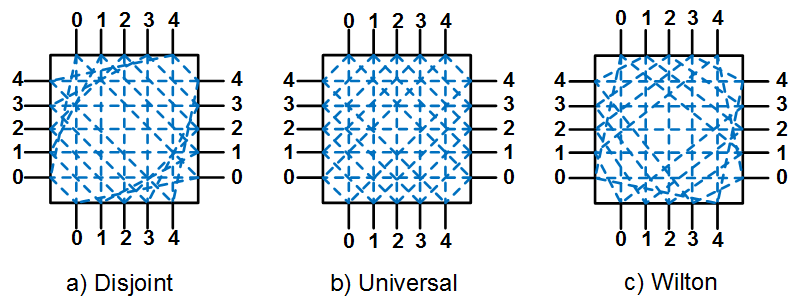
\includegraphics[width=0.33\textwidth]{fig/switchblocks.png}
    \caption{Wilton switch block pattern \cite{Yu2017FPGATargetability}}
    \label{fig:wiltonswitchblock}
\end{figure}

% Assume basics is talked about in background already
Regardless of the switch block pattern, a switch point within the switch block connects all four directions together, and is structured as in figure \ref{fig:switchblock}. Each switch point, depending on the switch architecture, can contain one or more switches.

% TODO: draw switch block.

A unidirectional switch architecture as seen in figure \ref{fig:uniswitch} is used as the baseline of our proposed work. We define a switch used inside a switch block as a switch point. In this case, the unidirectional switch point consists of four input and four output directions. For a given output direction, a 3:1 multiplexer is used to multiplex each of its three input directions together. Memory configuration bits are used to select the appropriate input direction for output. During configuration, these memory bits are written to only once.

% Bidirectional switch
% \begin{figure}[!htb]
% \centering
% \begin{circuitikz}[scale=0.4]
%     % mux
%     \draw (10,0) node[muxdemux, muxdemux def={Lh=4, Rh=1, NL=3, NB=0, NT=1, NR=1, w=2}, anchor=rpin 1](right_mux){};
%     \draw (-10,0) node[muxdemux, muxdemux def={Lh=1, Rh=4, NL=1, NB=0, NT=1, NR=3,w=2}, anchor=lpin 1](left_mux){};
%     \draw (0, -10) node[muxdemux, muxdemux def={Lh=1, Rh=4, NL=1, NB=0, NT=1, NR=3,w=2}, rotate=90, anchor=lpin 1](bot_mux){};
%     \draw (0, 10) node[muxdemux, muxdemux def={Lh=1, Rh=4, NL=1, NB=1, NT=0, NR=3,w=2}, rotate=-90, anchor=lpin 1](top_mux){};
%     % Buffers
%     \draw (right_mux.rpin 1) to[short] ++(1,0) node[ieeestd buffer port, anchor=in](right_buf){};
%     \draw (left_mux.lpin 1) to[short] ++(-1,0) node[ieeestd buffer port, xscale=-1, anchor=in](left_buf){};
%     \draw (bot_mux.lpin 1) to[short] ++(0,-1) node[ieeestd buffer port, anchor=in, rotate=-90](bot_buf){};
%     \draw (top_mux.lpin 1) to[short] ++(0,1) node[ieeestd buffer port, anchor=in, rotate=90](top_buf){};
%     \draw (right_buf.out) to[short,-o] ++(1,0);
%     \draw (top_buf.out) to[short,-o] ++(0,1);
%     \draw (left_buf.out) to[short,-o] ++(-1,0);
%     \draw (bot_buf.out) to[short,-o] ++(0,-1);
%     % Coordinates out of buf (WHEN MODIFYING SCALE THESE COORDINATES MAY NEED TO BE ADJUSTED)
%     \draw (right_buf.out) to[short] ++(0,-3.5) coordinate(right_out);
%     \draw (left_buf.out) to[short] ++(0,-3.5) coordinate(left_out);
%     \draw (top_buf.out) to[short] ++(3.5,0) coordinate(top_out);
%     \draw (bot_buf.out) to[short] ++(3.5,0) coordinate(bot_out);
%     % Horizontal lines + make dot coordinates
%     \draw (right_mux.lpin 1) to[short, -*] (right_mux.lpin 1 -| top_out) coordinate(dot1) to[short] (left_mux.rpin 1);
%     \draw (right_mux.lpin 2) to[short, -*]  (right_mux.lpin 2 -| top_mux.rpin 1) coordinate(dot2) to[short] (left_mux.rpin 2);
%     \draw (right_mux.lpin 3) to[short, -*] (right_mux.lpin 3 -| top_mux.rpin 2) coordinate(dot3);
%     % Vertical lines + make last dot coordinate
%     \draw (top_mux.rpin 3) to[short, -*] (top_mux.rpin 3 |- left_out) coordinate(dot4) to[short] (bot_mux.rpin 1);
%     \draw (top_mux.rpin 2) to[short] (bot_mux.rpin 2);
%     \draw (bot_mux.rpin 3) to[short] (dot2 |- dot1) to[short] ++(0,0.5) coordinate(t1);
%     \draw (top_mux.rpin 1) to[short] ++(0,-0.5) coordinate(t2);
%     % Buffer output coordinates to muxes
%     \draw (left_mux.rpin 3) to[short] ++(0.5,0) coordinate(r2);
%     \draw (right_out) to[short] (dot4) to[short] ++(-0.5,0) coordinate(r1) to[short] (r2);
%     \draw (left_out) to[short] (dot4 -| r2) to[short] (dot3 -| r1) to[short] (dot3);
%     \draw (bot_out) to[short] (dot1 |- t1) to[short] (t2);
%     \draw (top_out) to[short] (dot1 |- t2) to[short] (t1);
%     % SRAM boxes
%     \draw (top_mux.bpin 1) node [draw,align=center, anchor=e] {sram};
%     \draw (bot_mux.tpin 1) node [draw,align=center, anchor=e] {sram};
%     \draw (right_mux.tpin 1) node [draw,align=center, anchor=south] {sram};
%     \draw (left_mux.tpin 1) node [draw,align=center, anchor=south] {sram};    
% \end{circuitikz}
% \caption{Single bidirectional switch}
% \label{fig:biswitch}
% \end{figure}

% Unidirection switch
\begin{figure}[!htb]
\centering
\begin{circuitikz}[scale=0.4]
    % mux
    \draw (12,4) node[muxdemux, muxdemux def={Lh=4, Rh=1.5, NL=3, NB=0, NT=1, NR=1,w=1.5}, anchor=rpin 1](right_mux){};
    \draw (-12,-4) node[muxdemux, muxdemux def={Lh=1.5, Rh=4, NL=1, NB=0, NT=1, NR=3,w=1.5}, anchor=lpin 1](left_mux){};
    \draw (-4, -12) node[muxdemux, muxdemux def={Lh=1.5, Rh=4, NL=1, NB=0, NT=1, NR=3,w=1.5}, rotate=90, anchor=lpin 1](bot_mux){};
    \draw (4, 12) node[muxdemux, muxdemux def={Lh=1.5, Rh=4, NL=1, NB=1, NT=0, NR=3,w=1.5}, rotate=-90, anchor=lpin 1](top_mux){};
    % Buffers
    \draw (right_mux.rpin 1) to[short] ++(1,0) node[ieeestd buffer port, anchor=in,scale=0.75](right_buf){};
    \draw (left_mux.lpin 1) to[short] ++(-1,0) node[ieeestd buffer port, xscale=-1, anchor=in,scale=0.75](left_buf){};
    \draw (bot_mux.lpin 1) to[short] ++(0,-1) node[ieeestd buffer port, anchor=in, rotate=-90,scale=0.75](bot_buf){};
    \draw (top_mux.lpin 1) to[short] ++(0,1) node[ieeestd buffer port, anchor=in, rotate=90,scale=0.75](top_buf){};
    \draw (right_buf.out) to[short,-o] ++(1,0);
    \draw (top_buf.out) to[short,-o] ++(0,1);
    \draw (left_buf.out) to[short,-o] ++(-1,0);
    \draw (bot_buf.out) to[short,-o] ++(0,-1);
    % Drivers
    \draw (right_mux.lpin 1) 
    to[short, -*] (top_mux.rpin 3 |- right_mux.lpin 1) coordinate(r1)
    to[short, -*] (bot_mux.rpin 2 |- right_mux.lpin 1) coordinate(r0)
    to[short] (left_mux |- right_mux.lpin 1) coordinate (right_driver_out);
    \draw (right_driver_out) node[ieeestd buffer port, anchor=out,scale=0.5](right_driver){};
    \draw (right_driver.in) to[short,-o] ++(-1,0);   
    \draw (left_mux.rpin 3) 
    to[short, -*] (bot_mux.rpin 3 |- left_mux.rpin 3) coordinate(l1)
    to[short, -*] (top_mux.rpin 2 |- left_mux.rpin 3) coordinate(l0)
    to[short] (right_mux |- left_mux.rpin 3) coordinate (left_driver_out);
    \draw (left_driver_out) node[ieeestd buffer port, anchor=out,scale=0.5,xscale=-1](left_driver){};
    \draw (left_driver.in) to[short,-o] ++(1,0);
    \draw (bot_mux.rpin 1) 
    to[short, -*] (left_mux.rpin 1 -| bot_mux.rpin 1) coordinate(b1)
    to[short, -*] (right_mux.lpin 2 -| bot_mux.rpin 1) coordinate(b0)
    to[short] (top_mux -| bot_mux.rpin 1) coordinate (bot_driver_out);
    \draw (bot_driver_out) node[ieeestd buffer port, anchor=out,scale=0.5,rotate=-90](bot_driver){};
    \draw (bot_driver.in) to[short,-o] ++(0,1);
    \draw (top_mux.rpin 1) 
    to[short, -*] (right_mux.lpin 3 -| top_mux.rpin 1) coordinate(t1)
    to[short, -*] (left_mux.rpin 2 -| top_mux.rpin 1) coordinate(t0)
    to[short] (bot_mux -| top_mux.rpin 1) coordinate (top_driver_out);
    \draw (top_driver_out) node[ieeestd buffer port, anchor=out,scale=0.5,rotate=90](top_driver){};
    \draw (top_driver.in) to[short,-o] ++(0,-1);
    % Simple Connections
    \draw (top_mux.rpin 3) -- (r1);
    \draw (bot_mux.rpin 3) -- (l1);
    \draw (left_mux.rpin 1) -- (b1);
    \draw (right_mux.lpin 3) -- (t1);
    \draw (top_mux.rpin 2) -- (l0);
    \draw (bot_mux.rpin 2) -- (r0);
    \draw (left_mux.rpin 2) -- (t0);
    \draw (right_mux.lpin 2) -- (b0);
    % % SRAM boxes
    \draw (top_mux.bpin 1) node [draw,align=center, anchor=e] {sram};
    \draw (bot_mux.tpin 1) node [draw,align=center, anchor=e] {sram};
    \draw (right_mux.tpin 1) node [draw,align=center, anchor=south] {sram};
    \draw (left_mux.tpin 1) node [draw,align=center, anchor=south] {sram};      

\end{circuitikz}
\caption{Single unidirectional switch}
\label{fig:uniswitch}
\end{figure}

\subsection{Baseline multiplexer architecture}
\label{arch:mux_arch}
The number of configuration bits used within the unidirectional switch point's multiplexer can differ depending on its  circuitry.
There are two cases.
The first case is simple; the number of configuration bits used ties directly to the number of multiplexer inputs. For 3 multiplexer inputs, there are 3 configuration bits, as shown in figure \ref{fig:simple_mux}.
% TODO: change up the multiplexer SRAM bits because they are not just a single transistor in this diagram?
% Basic mux arch where 3 bits control 3 lines
\begin{figure}[!htb]
    \centering
    \begin{circuitikz}
        \draw (0,0) node[muxdemux, muxdemux def={Lh=4, Rh=1, NL=3, NB=0, NT=1, NR=1}](mux){};
        \draw (-2, 3) node[nmos](t1){};
        \draw (0, 3) node[nmos](t2){};
        \draw (2, 3) node[nmos](t3){};
        \draw (t1.S) to[short] ++(0,-0.25) to[short] ++(4,0);
        \draw (t2.S) to[short] ++(0,-0.25) to[short] ++(0,0);
        \draw (t3.S) to[short] ++(0,-0.25) to[short] ++(0,0);
        \draw (mux.tpin 1) to[short] ++(0,1);
        \draw (t1.D) to[short, -o] ++(0,.25);
        \draw (t2.D) to[short, -o] ++(0,.25);
        \draw (t3.D) to[short, -o] ++(0,.25);
    \end{circuitikz}
    \caption{Simple multiplexer using 3 configuration memory bits}
    \label{fig:simple_mux}
\end{figure}

The second case reduces the number of configuration bits by using an intermediate decoder. The decoder in figure \ref{fig:decoder_new} allows compressing the number of input directions by $log_2$. 2 configuration bits can be used to control 4 input lines, shown in figure \ref{fig:decoder_mux}. We consider this structure as the baseline as it minimizes the number of configuration memory bits.
% the existing circuitry used to read/write to the two configuration memory bits of a bidirectional track can be used to read/write to the two configuration memory bits of an unidirectional track. Further, since the unidirectional track splits up the bidirectional track in two. This is shown in figure \ref{fig:proposed_arch}. 

% Decoder_mux
\begin{figure}[!htb]
    \centering
    \begin{circuitikz}
        \draw (0,0) node[muxdemux, muxdemux def={Lh=4, Rh=1, NL=3, NB=0, NT=1, NR=1}](mux){};
        \draw (-1, 5) node[nmos](t1){};
        \draw (1, 5) node[nmos](t3){};
        \draw (t1.S) to[short] ++(0,-0.25) to[short] ++(2,0);
        \draw (t3.S) to[short] ++(0,-0.25) to[short] ++(0,0);
        \draw (mux.tpin 1) to[short] ++(0,1) node [draw,align=center, anchor=south](dec) {decoder};
        \draw (dec.north) to[short] ++(0,1.47);
        \draw (t1.D) to[short, -o] ++(0,.25);
        \draw (t3.D) to[short, -o] ++(0,.25);
    \end{circuitikz}
    \caption{2 bits of configuration memory using a decoder + 3:1 multiplexer}
    \label{fig:decoder_mux}
\end{figure}

4 decoder outputs are possible with two bits of configuration memory, although in the baseline unidirectional switch configuration only 3 are used since there are 3 inputs into the multiplexer. We assume there exists a 4th input as ground, since it is unlikely that during normal switch point operation all outputs are driven regardless of use.

\begin{figure}[!htb]
    \centering
    \begin{circuitikz}
        \draw (1,0.5) node [draw, align=center, anchor=south](sram){sram[1:0]};
        \draw (0,0) to[short, o-] ++(0,-1) node[ieeestd not port, rotate=-90, anchor=in](not1){};       
        \draw (2,0) to[short, o-] ++(0,-1) node[ieeestd not port, rotate=-90, anchor=in](not2){};
        % First and gate
        \draw (not2.out) to[short, -*] ++(0,-1) to[short] ++(1,0) node[ieeestd and port, anchor=in 1](and1){}; 
        \draw (not1.out) to[short, -*] ++(0,-1.56) to[short] (and1.in 2);
        % Second and gate
        \draw (not2.in) to[short] ++(-1,0) to[short,-*] ++(0,-4.5)  coordinate(and4_start1) to[short] ++(2,0)  node[ieeestd and port, anchor=in 1](and2){};
        \draw (not1.out) to[short] ++(0,-3.3) to[short] (and2.in 2);
        % Third and gate
        \draw (not1.in) to[short] ++(-1,0) to[short,-*] ++(0,-6.25)  coordinate(and4_start2) to[short] ++(4,0)  node[ieeestd and port, anchor=in 1](and3){};
        \draw (not2.out) to[short] ++(0,-5.06) to[short] (and3.in 2);
        % Fourth and gate
        \draw (and4_start1) to[short] ++(0,-3.5) to[short] ++(2,0) node[ieeestd and port, anchor=in 1](and4){};
        \draw (and4_start2) to[short] (and4_start2 |- and4.in 2) to[short] (and4.in 2);
    \end{circuitikz}
        \caption{2:4 decoder structure}
    \label{fig:decoder_new}
\end{figure}

% Note that in regards to area, the number of transistors for the multiplexer decoder is the same for the unmodified baseline versus with the proposed circuitry, since the decoder circuitry is not modified.

\section{The bidirectional track architecture}
\label{arch:limitations}
% Limitations of baseline, including that it was done on older technology and bidirectional wires.
% Section \ref{bg:wideshallowmem} provides an introductory background into prior work. 
This section details the bidirectional track architecture and how it is used in prior work for comparison with the proposed architecture in the following section \ref{arch:proposed}. 

A bidirectional switch point considered in prior work as seen in figure \ref{fig:bidirectional_switchpoint}, has 1 horizontal connection, 1 vertical connection, and 4 diagonal connections for a total of 6 connections possible. All of these connections are implemented within a switch point. Each switch connection (figure \ref{fig:prior_baseline} consists of a bidirectional driver made up of 2 tri-state buffers. Each tri-state is controlled by one configuration bit memory. In prior work, the horizontal and vertical connections are used and left unmodified to allow for memory input and output of the switch point to connect to the switch block external pins. The 4 diagonal connections are modified to access the 2 configuration bits. In the original baseline, the 4 diagonal connections' configuration bits would be unused when the horizontal and vertical connections are used.

Prior work's bidirectional switch architecture, depicted in figure \ref{fig:prior_arch}, modifies the baseline bidirectional switch (figure \ref{fig:prior_baseline} to take advantage of the unused configuration memory within these diagonal connections. By adding pass transistors to the switch, the configuration memory can be both read out and written to. More specifically, disconnecting the diagonal connections is made possible by adding, then turning off, a pass transistor in the critical path of the bidirectional connection as seen in figure \ref{fig:prior_arch}.

Figure \ref{fig:prior_control} shows prior work's memory addressing and control circuitry. As mentioned, the vertical and horizontal switches cannot be used as memory since the tracks they implement are used to connect to the address decoder or to access the configuration memory. This means that only the diagonal connections are able to be read and written to. Further, this makes up 8 bits of accessible memory per switch point and corresponds to a memory depth of 8.  The lower right of figure \ref{fig:prior_control} shows the disconnected 4 diagonal connections possible that allow for memory to be read out or written to. Since only the diagonal switches within a switch block are modified to allow for access in all directions, all non-diagonal switches are kept in its vertical and horizontal connection configuration, allowing for this connection. Lastly, the tri-state drivers in the horizontal and vertical track directly turn off unused inputs and outputs, reducing power.

% Prior arch
\begin{figure}[!htb]
\begin{center}
\begin{circuitikz}[scale=1]
    % Pass transistor + sram write transistor
    \draw (0, 0) node[nmos, rotate=-90](p1){} ++(0,1) to[short] ++(0,1) node[nmos, anchor=S](t1){};
    % sram sel transistor
    \node [nmos,rotate=-90,anchor=D](t2) at (t1.D){};
    % sram Inverters
    \node [ieeestd not port, anchor=in](a1) at (t1.D){};
    \node [ieeestd not port, rotate=-180, anchor=out](a2) at (t1.S){};
    % Connect sram inverters
    \draw (a2.in) to (a1.out);
    % sram Labels
    \draw (t1.G) to[short,l=write] ++(0,0);
    \draw (t2.G) to[short,l=select] ++(0,0);
    \draw (t2.S) to[short,l=to config lines] ++(0,0);
    % Tri state
    \node[blue] [nmos, rotate=-90, anchor=D](p3) at (p1.S){};
    \node [ieeestd not port, anchor=out](a3) at (p3.S){};
    \node [ieeestd not port, anchor=out](a4) at (a3.in){};
    \draw (a4.in) to[short] ++(0,-2);
    \draw (p1.D) to[short] ++(0,-2) node[ieeestd not port, xscale=-1,anchor=in](a5){};
    \node [ieeestd not port, xscale=-1, anchor=in](a6) at (a5.out){};
    \node[blue] [nmos, rotate=90, anchor=S](p4) at (a6.out){};
    \node [nmos, rotate=90, anchor=S](p2) at (p4.D){};
    % Draw 2nd sram below
    \draw (p2.G) to[short] ++(0,-1) node[nmos, xscale=-1, anchor=D](t3){};
    % sram sel transistor
    \node [nmos,rotate=-90,xscale=-1,anchor=S](t4) at (t3.S){};
    % sram Inverters
    \node [ieeestd not port,anchor=out](a3) at (t3.D){};
    \node [ieeestd not port,xscale=-1,anchor=in](a4) at (t3.S){};
    % Connect sram inverters
    \draw (a3.in) to (a4.out);
    % sram Labels
    \draw (t3.G) to[short,l=write] ++(0.3,0);
    \draw (t4.G) to[short,l=select] ++(0,0);
    \draw (t4.D) to[short,l=to config lines] ++(1,0);
    % transistor labels
    \draw[blue] (p3.G) to[short, l=!M] ++(0,0);
    \draw[blue] (p4.G) to[short, l=!M] ++(0,0);
    % to other tracks
    \draw[blue] (t1.D) to[short] ++(0,1) to[short] ++(2,0) node[nmos, rotate=-90,anchor=S](w1){};
    \draw[blue] (w1.D) to[short] ++(0.5,0) to[short] ++(0,-3) node[nmos, rotate=-90, anchor=S](w2){};
    \draw[blue] (w2.G) ++(2,0) to[short,l=MemVert] ++(0,0);
    \draw[blue] (w2.D) ++(2.5,0) to[short, l=vertical track] ++(0,0);
    \draw[blue] (w2.S) to[short] ++(0,-3) node[nmos, rotate=-90, anchor=S](w3){};
    \draw[blue] (w3.D) ++(3,0) to[short, l=horizontal track] ++(0,0);
    \draw[blue] (w3.G) ++(2,0) to[short,l=MemHorz] ++(0,0);
    \draw[blue] (t4.S) to[short] ++(0,-2) to[short] ++(7,0) node[nmos, rotate=-90,anchor=S](w4){};
    \draw[blue] (w4.D) to[short] ++(0.525,0) to[short] (w3.S);
    \draw[blue] (w1.G) to[short, l=AS1] ++(0,0);
    \draw[blue] (w4.G) to[short, l=AS2] ++(0,0);
    \end{circuitikz}
\caption{Prior work's bidirectional connection, enhanced programmable connection in blue}
\label{fig:prior_arch}
\end{center}
\end{figure}

% Prior work's control/address circuitry figure
\begin{figure}[!htb]
\begin{center}
\begin{circuitikz}[scale=1]
    % Decoder
    \draw (0,0) node[muxdemux, muxdemux def={Lh=8, Rh=8, w=4, NL=8, NB=3, NT=0, NR=0}, anchor=lpin 1](decoder){3:8 decoder};
    % Decoder labels
    \draw (decoder.lpin 3) to[short, l=AS1(3..0)] ++(0,0);
    \draw (decoder.lpin 6) to[short, l=AS2(3..0)] ++(0,0);
    % Address labels
    \draw (decoder.bpin 1) ++(0,-0.5) to[short, l=A0] ++(0,0);
    \draw (decoder.bpin 2) ++(0,-0.5) to[short, l=A1] ++(0,0);
    \draw (decoder.bpin 3) ++(0,-0.5) to[short, l=A2] ++(0,0);
    % Address pins
    \draw (decoder.bpin 1) to[short] ++(0,-4) coordinate(h1);
    \draw (decoder.bpin 2) to[short] ++(0,-4) coordinate(h2);
    \draw (decoder.bpin 3) to[short] ++(0.25,0) to[short] ++(0,-1) coordinate(a2in);
    % A2 and lines
    \draw (a2in) node[muxdemux, muxdemux def={Lh=2, Rh=1, w=1, NL=2, NB=1, NT=0, NR=1}, anchor=rpin 1, rotate=90](a2mux){};
    \draw (a2mux.bpin 1) ++(1,0) to[short,l=bit 2] ++(0,0);
    % Vertical track
    \draw (a2mux.lpin 2) 
    to[short]       ++(2  ,0) coordinate(v0)
    to[short, -*]   ++(0.5,0) coordinate(v1) 
    to[short]       ++(0.5,0) coordinate(v2) 
    to[short]       ++(0.5,0) coordinate(v3) 
    to[short]       ++(0.5,0) coordinate(v4)
    to[short, -*]   ++(0.5,0) coordinate(v5)
    to[short]       ++(0.5,0) coordinate(v6)
    to[short]       ++(0.5,0) coordinate(v7)
    to[short]       ++(0.5,0) coordinate(v8)
    to[short]       ++(0.25,0) coordinate(v9);
    \draw (v0) 
    to[short, -*]   ++(0, -0.5) coordinate(vl0)
    to[short]       ++(0, -0.25) coordinate(arrow1)
    to[short]       ++(0, 0.75) coordinate(vl1)
    to[short]       ++(0, 0.5)  coordinate(vl2)
    to[short]       ++(0, 0.5)  coordinate(vl3)
    to[short]       ++(0,3);
    \draw (v1) 
    to[short]       ++(0, -0.5)
    to[short]       ++(0, -0.25) 
    to[short]       ++(0, 0.75)
    to[short]       ++(0, 0.5)
    to[short]       ++(0, 0.5)
    to[short]       ++(0,3);
    \draw (v2) 
    to[short]       ++(0, -0.5)
    to[short]       ++(0, -0.25) coordinate(line0)
    to[short]       ++(0, 0.75)
    to[short, -*]   ++(0, 0.5)
    to[short]       ++(0, 0.5)
    to[short]       ++(0,3);
    \draw (v3) 
    to[short]       ++(0, -0.5)
    to[short]       ++(0, -0.25) 
    to[short]       ++(0, 0.75)
    to[short]       ++(0, 0.5)
    to[short, -*]   ++(0, 0.5)
    to[short]       ++(0,3);
    \draw (v4) 
    to[short, -*]   ++(0, -0.5)
    to[short]       ++(0, -0.25) coordinate(line1)
    to[short]       ++(0, 0.75)
    to[short]       ++(0, 0.5)
    to[short]       ++(0, 0.5)
    to[short]       ++(0,3);
    \draw (v5) 
    to[short]       ++(0, -0.5)
    to[short]       ++(0, -0.25) coordinate(arrow2)
    to[short]       ++(0, 0.75)
    to[short]       ++(0, 0.5)
    to[short]       ++(0, 0.5)
    to[short]       ++(0,3);
    \draw (v6) 
    to[short]       ++(0, -0.5)
    to[short]       ++(0, -0.25) 
    to[short]       ++(0, 0.75)
    to[short,-*]    ++(0, 0.5)
    to[short]       ++(0, 0.5)
    to[short]       ++(0,3);
    \draw (v7) 
    to[short]       ++(0, -0.5)
    to[short]       ++(0, -0.25) 
    to[short]       ++(0, 0.75)
    to[short]       ++(0, 0.5)
    to[short,-*]    ++(0, 0.5)
    to[short]       ++(0,3);
    \draw (v8) 
    to[short]       ++(0, -0.5) coordinate(ve0)
    to[short]       ++(0, -0.25)
    to[short]       ++(0, 0.75) coordinate(ve2)
    to[short]       ++(0, 0.5)  coordinate(ve3)
    to[short]       ++(0, 0.5)  coordinate(ve4)
    to[short]       ++(0,3) ++(0,0.5) to[short, l=Vertical routing tracks] ++(0,0);
    \draw (vl0) to[short] (ve0) to[short] ++(0.25,0);
    \draw (vl1) to[short] (ve2) to[short] ++(0.25,0);
    \draw (vl2) to[short] (ve3) to[short] ++(0.25,0);
    \draw (vl3) to[short] (ve4) to[short] ++(0.25,0);
    % Horizontal track
    \draw (a2mux.lpin 1) to[short] (h2 -| a2mux.lpin 1) coordinate(h3);
    \draw (h2) to[short] ++(2.5,0) coordinate(arrow1end) to[short] ++(4,0) coordinate(hend); 
    \draw (h2) to[short, -*] ++(-1.5,0) coordinate(h0) to[short] ++(-3,0) coordinate(hstart);
    \draw (h0) to[short] ++(0,-0.5) coordinate(l1)
    to[short] ++(0,-0.5) coordinate(l2)
    to[short] ++(0,-0.5) coordinate(l3)
    to[short, -*] ++(0,-0.5) coordinate(l4)
    to[short] ++(0,-0.5) coordinate(l5)
    to[short] ++(0,-0.5) coordinate(l6)
    to[short] ++(0,-0.5) coordinate(l7)
    to[short] ++(0,-0.5) coordinate(l8)
    to[short] ++(0,-0.5) coordinate(l9);
    \draw (h1) to[short] (l9 -| h1);
    \draw (h2) to[short] (l9 -| h2);
    \draw (h3) to[short] (l9 -| h3);
    \draw (l1) to[short, -*] (l1 -| h1) to[short] ++(2,0) coordinate(hend1);
    \draw (l1) to[short] (l1 -| hstart);
    \draw (l2) to[short, -*] (l2 -| h2) to[short] (l2 -| hend1);
    \draw (l2) to[short] (l2 -| hstart);
    \draw (l3) to[short, -*] (l3 -| h3) to[short] (l3 -| hend1);
    \draw (l3) to[short] (l3 -| hstart);
    \draw (l4) to[short, -*] (l4 -| h0) to[short] (l4 -| hend1);
    \draw (l4) to[short] (l4 -| hstart);
    \draw (l5) to[short, -*] (l5 -| h1) to[short] (l5 -| hend1);
    \draw (l5) to[short] (l5 -| hstart);
    \draw (l6) to[short, -*] (l6 -| h2) to[short] (l6 -| hend1);
    \draw (l6) to[short] (l6 -| hstart);
    \draw (l7) to[short, -*] (l7 -| h3) to[short] (l7 -| hend1);
    \draw (l7) to[short] (l7 -| hstart);
    \draw (l8) to[short, -*] (l8 -| h0) to[short] (l8 -| hend1);
    \draw (l8) to[short] (l8 -| hstart)
    ++(3, -0.5)to[short, l=Horizontal routing tracks] ++(0,0);
    % Circuitry
    \draw (h0) to[short] ++(0,2) to[short] ++(-2,0) node[ieeestd xor port, anchor=in 1, xscale=-1,scale=0.5](xor){};
    \draw (xor.in 2) ++(1,-0.05) to[short, l=bit 2] ++(0,0);
    \draw (xor.out) to[short] ++(-0.25,0) to[short] ++(0,0.25) node[ieeestd and port, anchor=in 2, rotate=90, scale=0.5](and){};
    \draw(and.out) to[short] ++(0,1.1) ++(0,0) to[short, l=MemVert] ++(0,0);
    \draw (and.out) to[short] ++(0.5,0) node[ieeestd not port, anchor=in, rotate=90,scale=0.5](not0){};
    \draw (not0.out) to[short] ++(0,0.25) ++(2,0) to[short,l=MemHorz] ++(0,0);
    \draw (and.in 1) to[short] ++(0,-1.5) to[short,l=bit 1] ++(0,0);
    \draw (and.in 1) to[short] ++(0,-0.5) to[short] ++(-1,0) to[short] ++(0,0.25) node[ieeestd not port, anchor=in, rotate=90, scale=0.5](not1){};
    \draw (not1.out) to[short,l=!M] ++(0,0);
    % Arrows
    \draw [latexslim-latexslim,scale=2] (arrow1) -- (arrow1end);
    \draw [latexslim-latexslim,scale=2] (arrow2) -- (hend);
    \draw (line0) ++(0,-2) coordinate(arrow3);
    \draw (arrow3) to[short] ++(0,-1);
    \draw (line1) ++(0,-2) coordinate(arrow4);
    \draw (arrow4) to[short] ++(0,-1);
    \draw [latexslim-latexslim,scale=2] (arrow3) -- (hend);
    \draw [latexslim-latexslim,scale=2] (arrow4) -- (arrow1end);

    \end{circuitikz}
\caption{Prior work's addressing and control circuitry, only the A2 multiplexer is shown for simplicity}
\label{fig:prior_control}
\end{center}
\end{figure}

For each switch block the memory is made addressable by delegating 3 track lines as address lines. This controls the AS1 and AS2 pass transistors. Following these address transistors is an intermediate staging area, connected to the horizontal and vertical track via two more pass transistors controlled using 1 control line. In total, 4 track lines comprises A0-A2 (for a memory depth of 8 since $log_2(8)=3$) and a control line to select MemVert, MemHorz, and M. MemVert and MemHorz control the input/output track direction while M selects usage of the switch block as a memory or regular switch block and is controlled by bit 1. Bit 1 and 2 come from two configuration bits, a necessary overhead per switch block. Bit 2 controls the logic that selects between a horizontal track input or vertical track input. Accordingly, if used as memory, the output is selected to be the other track. 
This allows for memory access to the now user-accessible memories within these diagonal switches. 
% Since these drivers no longer form a loop within the same switch, much more flexibility can be added into the memory addressing and control. This can be seen by comparing address and control circuitry.

However, the configuration memory made accessible in prior work specifically targets a bidirectional architecture using tri-state inverters. In more modern architectures, the tri-state buffers are removed in favour for multiplexers in a unidirectional manner. Since prior work modifies the architecture of the tri-state buffers within the switch block to be able to be read out and written to, this can no longer be feasible. 

\section{The unidirectional switch (and why directly mapping prior work doesn't work)}
% TODO: include in overhead calculation
In a unidirectional switch, instead of reading and writing to the tri-state buffer's configuration memory, the multiplexer's configuration memory is used instead. Seen in figure \ref{fig:uniswitch}, this configuration memory is used to multiplex one of three incoming input directions to its output direction. The fourth input direction (not-depicted) is connected to ground when not in use.

\begin{figure}
    \begin{circuitikz}
% left tracks
    \draw(1,0) to[short,-o] (5,0) coordinate(l0);
    \draw(1,1) to[short,-o] (4,1) coordinate(l1);
    \draw(1,2) to[short,-o] (3,2) coordinate(l2);
    \draw(1,3) to[short,-o] (2,3) coordinate(l3);
% right tracks
    \draw(7,0) to[short,-o] (6,0) coordinate(r0);
    \draw(7,1) to[short,-o] (5,1) coordinate(r1);
    \draw(7,2) to[short,-o] (4,2) coordinate(r2);
    \draw(7,3) to[short,-o] (3,3) coordinate(r3);
% bot tracks
    \draw(5.5,-1) to[short,-o] (5.5,-0.5) coordinate(b0);
    \draw(4.5,-1) to[short,-o] (4.5,0.5) coordinate(b1);
    \draw(3.5,-1) to[short,-o] (3.5,1.5) coordinate(b2);
    \draw(2.5,-1) to[short,-o] (2.5,2.5) coordinate(b3);
% top tracks
    \draw(5.5,4) to[short,-o] (5.5,0.5)coordinate(t0);
    \draw(4.5,4) to[short,-o] (4.5,1.5)coordinate(t1);
    \draw(3.5,4) to[short,-o] (3.5,2.5)coordinate(t2);
    \draw(2.5,4) to[short,-o] (2.5,3.5)coordinate(t3);

% Direct connections
\draw[blue] (l0) to[short] (r0);
\draw[blue] (l1) to[short] (r1);
\draw[blue] (l2) to[short] (r2);
\draw[blue] (l3) to[short] (r3);
\draw[blue] (t0) to[short] (b0);
\draw[blue] (t1) to[short] (b1);
\draw[blue] (t2) to[short] (b2);
\draw[blue] (t3) to[short] (b3);
% Diagonal connections
\draw[blue, densely dotted] (l0) to[short] (t0);
\draw[blue, densely dotted] (l1) to[short] (t1);
\draw[blue, densely dotted] (l2) to[short] (t2);
\draw[blue, densely dotted] (l3) to[short] (t3);
\draw[blue, densely dotted] (t0) to[short] (r0);
\draw[blue, densely dotted] (t1) to[short] (r1);
\draw[blue, densely dotted] (t2) to[short] (r2);
\draw[blue, densely dotted] (t3) to[short] (r3);
\draw[blue, densely dotted] (r3) to[short] (b3);
\draw[blue, densely dotted] (r2) to[short] (b2);
\draw[blue, densely dotted] (r1) to[short] (b1);
\draw[blue, densely dotted] (r0) to[short] (b0);
\draw[blue, densely dotted] (b0) to[short] (l0);
\draw[blue, densely dotted] (b1) to[short] (l1);
\draw[blue, densely dotted] (b2) to[short] (l2);
\draw[blue, densely dotted] (b3) to[short] (l3);

% Switch block outline
\draw[red, thick] (1.5,-0.75) to[short] (6.5,-0.75) to[short] (6.5,3.75) to[short] (1.5,3.75) to[short] (1.5,-0.75);
    \end{circuitikz}
\caption{Bidirectional switch points (blue) within a switch block (red), where each switch point is capable of 6 switch connections}
\label{fig:bidirectional_switchpoint}
\end{figure}

\begin{figure}
 \begin{circuitikz}
% left tracks
    \draw(1,0) to[short,-*] (5,0) coordinate(l00);
    \draw(1,0.5) to[short,-o] (5,0.5) coordinate(l0);
    \draw(1,1) to[short,-*] (4,1) coordinate(l11);
    \draw(1,1.5) to[short,-o] (4,1.5) coordinate(l1);
    \draw(1,2) to[short,-*] (3,2) coordinate(l22);
    \draw(1,2.5) to[short,-o] (3,2.5) coordinate(l2);
    \draw(1,3) to[short,-*] (2,3) coordinate(l33);
    \draw(1,3.5) to[short,-o] (2,3.5) coordinate(l3);
% right tracks
    \draw(7,0) to[short,-o] (6,0) coordinate(r0);
    \draw(7,0.5) to[short,-*] (6,0.5) coordinate(r00);
    \draw(7,1) to[short,-o] (5,1) coordinate(r1);
    \draw(7,1.5) to[short,-*] (5,1.5) coordinate(r11);
    \draw(7,2) to[short,-o] (4,2) coordinate(r2);
    \draw(7,2.5) to[short,-*] (4,2.5) coordinate(r22);
    \draw(7,3) to[short,-o] (3,3) coordinate(r3);
    \draw(7,3.5) to[short,-*] (3,3.5) coordinate(r33);
% bot tracks
    \draw(5.25,-0.75) to[short,-o] (5.25,-0.25) coordinate(b0);
    \draw(4.25,-0.75) to[short,-o] (4.25,0.75) coordinate(b1);
    \draw(3.25,-0.75) to[short,-o] (3.25,1.75) coordinate(b2);
    \draw(2.25,-0.75) to[short,-o] (2.25,2.75) coordinate(b3);
    \draw(5.75,-0.75) to[short,-*] (5.75,-0.25) coordinate(b00);
    \draw(4.75,-0.75) to[short,-*] (4.75,0.75) coordinate(b11);
    \draw(3.75,-0.75) to[short,-*] (3.75,1.75) coordinate(b22);
    \draw(2.75,-0.75) to[short,-*] (2.75,2.75) coordinate(b33);
% top tracks
    \draw(5.75,4.25) to[short,-o] (5.75,0.75)coordinate(t0);
    \draw(4.75,4.25) to[short,-o] (4.75,1.75)coordinate(t1);
    \draw(3.75,4.25) to[short,-o] (3.75,2.75)coordinate(t2);
    \draw(2.75,4.25) to[short,-o] (2.75,3.75)coordinate(t3);
    \draw(5.25,4.25) to[short,-*] (5.25,0.75)coordinate(t00);
    \draw(4.25,4.25) to[short,-*] (4.25,1.75)coordinate(t11);
    \draw(3.25,4.25) to[short,-*] (3.25,2.75)coordinate(t22);
    \draw(2.25,4.25) to[short,-*] (2.25,3.75)coordinate(t33);

% Direct connections
\draw[blue] (l0) to[short] (r00);
\draw[blue] (l1) to[short] (r11);
\draw[blue] (l2) to[short] (r22);
\draw[blue] (l3) to[short] (r33);
\draw[blue] (t0) to[short] (b00);
\draw[blue] (t1) to[short] (b11);
\draw[blue] (t2) to[short] (b22);
\draw[blue] (t3) to[short] (b33);
\draw[blue] (l00) to[short] (r0);
\draw[blue] (l11) to[short] (r1);
\draw[blue] (l22) to[short] (r2);
\draw[blue] (l33) to[short] (r3);
\draw[blue] (t00) to[short] (b0);
\draw[blue] (t11) to[short] (b1);
\draw[blue] (t22) to[short] (b2);
\draw[blue] (t33) to[short] (b3);
% Diagonal connections
\draw[blue, densely dotted] (l0) to[short] (t00);
\draw[blue, densely dotted] (l1) to[short] (t11);
\draw[blue, densely dotted] (l2) to[short] (t22);
\draw[blue, densely dotted] (l3) to[short] (t33);
\draw[blue, densely dotted] (t0) to[short] (r00);
\draw[blue, densely dotted] (t1) to[short] (r11);
\draw[blue, densely dotted] (t2) to[short] (r22);
\draw[blue, densely dotted] (t3) to[short] (r33);
\draw[blue, densely dotted] (r3) to[short] (b33);
\draw[blue, densely dotted] (r2) to[short] (b22);
\draw[blue, densely dotted] (r1) to[short] (b11);
\draw[blue, densely dotted] (r0) to[short] (b00);
\draw[blue, densely dotted] (b0) to[short] (l00);
\draw[blue, densely dotted] (b1) to[short] (l11);
\draw[blue, densely dotted] (b2) to[short] (l22);
\draw[blue, densely dotted] (b3) to[short] (l33);
\draw[blue, densely dotted] (l00) to[short] (t0);
\draw[blue, densely dotted] (l11) to[short] (t1);
\draw[blue, densely dotted] (l22) to[short] (t2);
\draw[blue, densely dotted] (l33) to[short] (t3);
\draw[blue, densely dotted] (t00) to[short] (r0);
\draw[blue, densely dotted] (t11) to[short] (r1);
\draw[blue, densely dotted] (t22) to[short] (r2);
\draw[blue, densely dotted] (t33) to[short] (r3);
\draw[blue, densely dotted] (r33) to[short] (b3);
\draw[blue, densely dotted] (r22) to[short] (b2);
\draw[blue, densely dotted] (r11) to[short] (b1);
\draw[blue, densely dotted] (r00) to[short] (b0);
\draw[blue, densely dotted] (b00) to[short] (l0);
\draw[blue, densely dotted] (b11) to[short] (l1);
\draw[blue, densely dotted] (b22) to[short] (l2);
\draw[blue, densely dotted] (b33) to[short] (l3);

% Switch block outline
\draw[red, thick] (1.5,-0.5) to[short] (6.5,-0.5) to[short] (6.5,4) to[short] (1.5,4) to[short] (1.5,-0.5);
    \end{circuitikz}
\caption{Unidirectional switch points (blue) within a switch block (red), where each switch is capable of 8 switch connections}
\label{fig:unidirectional_switchpoint}
\end{figure}

A unidirectional switch point, seen in figure \ref{fig:uniswitch} and figure \ref{fig:unidirectional_switchpoint}, has the possibility of 2 horizontal connections, 2 vertical connections, and 8 diagonal connections for a total of 12 possible switch connections. In contrast to the bidirectional switch point, not all connections are used, since the multiplexer selection results in only 8 connections connected at a time. As a result of the multiplexer simplifying and consolidating the total number of connections used, disconnecting only the 4 diagonal connections as done in prior work to allow for configuration memory access is no longer possible. Keeping the horizontal and vertical tracks in a normal usage configuration would mean that all 4 multiplexers are configured, leaving no possibility for any configuration memory to be open for access. This is effectively an unmodified unidirectional switch point. 

% and to minimize changes to this control circuit we can mimic the same structure of the bidirectional switch and assume that all horizontal (and all vertical) tracks are connected and staggered in the same way as in prior work. 

That being said, the unidirectional switch opens up a larger possibility of configuration memory switch structures. In prior work's bidirectional switch point, the diagonal switch connections are used as configuration memory.
This limits the possible input/output track choices to two. If the horizontal switch track is chosen to be the input, the other vertical switch track must be an output, and vice-versa.
On the other hand, the unidirectional switch allows for a finer selection granularity between the input and output track choices, since the input and output tracks are decoupled. This results in a possible total number of input/output track permutations of 16, because for every one (of four) input directions there are 4 output direction tracks possible. 
% Future work: although preserving the same diagonal structure is possible, there is no limitation to using diagonal switch points 

Therefore, having an input and output coming and leaving in any of the four directions is possible. An input and output coming from the same direction should be made possible, although unlikely in practice due to issues such as congestion. In order to keep such flexibility the proposed architecture must also be highly flexible. This also makes multi-ported memory possible, with multiple inputs or outputs. For sake of simplicity however we will consider only single-ported memory since additional circuitry to control multi-ported behaviour is much more complicated and adds extra overhead.

This flexibility increases the number of permutations further by varying the amount of user accessible configuration bits per switch point. Each multiplexer within the switch point has two bits of configuration memory, which can be either configured as user-accessible, leaving the multiplexer unused, or configured as normal operation, allowing for normal routing purposes. The use of such a hybrid configuration could potentially alleviate routing problems in the CAD flow. 

Exploring such an exhaustive list of the possible input/output memory switch connections along with varying the number of user accessible memory configurations can be left as future work as an architecture exploration, tying into a possible CAD framework tool. That being said, for this work we elucidate a possible subset of these configurations and select one that best fits the needs for a machine learning circuit context. 

Because we want to maximize memory, the number of user-accessible configuration bits should be maximized. Further, the enhanced memory connection of the switch block should be as flexible as possible, allowing for connections in all directions. A sweep of the number of bits per switch point versus minimum width transistor count is done in section \ref{arch:proposed} after the proposed architecture is explained.

Further, we assume a maximum of memory depth of 8 addresses since this is the maximum addressable range inside a single switch point, but it could be possible to connect the staging areas of multiple switch points together in order to achieve a deeper but less-wide memory block. 

Lastly, a modified input and output memory-to-track connection is needed in addition to a modified address and control circuitry. Since this is no longer a bidirectional connection, 2 pass transistors (ie. MemVert, MemHorz from prior work) cannot be used to connect to the input and output tracks.
% Additionally, the input and output tracks are decoupled from one another, so the address and control circuitry no longer takes up entire switch points.

% Insert picture of output in all directions
% Insert picture of output in some directions
% Talk about staggered connection instead of all directions

% To simplify architecture exploration, one assumption that can be made is to pair the opposite direction track pairs together. 

\section{Proposed architecture}
\label{arch:proposed}
The proposed architecture for a flexible, unidirectional, user-accessible switch point is shown in \ref{fig:proposed_arch}. 

% Proposed arch figure
\begin{figure}[!htb]
\begin{center}
\begin{circuitikz}[scale=1]
    % Base multiplexer
    \draw (0, 0) coordinate(base);
    % Write transistors
    \draw (base) to[short] ++(3,0) coordinate(base_right) to[short] ++(0,1) node[nmos, anchor=S](wrt1){};
    \draw (base) to[short] ++(-3,0) to[short] ++(0,1) node[nmos, anchor=S, xscale=-1](wrt2){};
    % sel transistor
    \node [nmos,rotate=-90,anchor=D](selt1) at (wrt1.D){};
    \node [nmos,rotate=90,anchor=D, xscale=-1](selt2) at (wrt2.D){};
    % sram Inverters
    \node [ieeestd not port, anchor=in](a1) at (wrt1.D){};
    \node [ieeestd not port, rotate=-180, anchor=out](a2) at (wrt1.S){};
    \node [ieeestd not port, anchor=in, xscale=-1](a3) at (wrt2.D){};
    \node [ieeestd not port, rotate=-180, anchor=out, xscale=-1](a4) at (wrt2.S){};
    % Connect sram inverters
    \draw (a2.in) to (a1.out);
    \draw (a4.in) to (a3.out);
    % sram Labels
    \draw (wrt1.G) to[short] ++(-0.5,0) ++(-1,0) to[short,l=write] ++(0,0);
    \draw (wrt2.G) to[short] ++(0.5,0);
    \draw (selt1.G) to[short] ++(-1,0) ++(-0.625,0) to[short,l=select] ++(0,0);
    \draw (selt2.G) to[short] ++(1,0);
    \draw (selt1.S) ++(-0.1,0) to[short,l=to config lines] ++(0,0);
    % to other tracks
    \draw[blue] (wrt1.D) to[short] ++(0,2) to[short] ++(2,0) node[nmos, rotate=-90,anchor=S](w1){};
    \draw[blue] (w1.G) to[short, l=AS1] ++(0,0);
    \draw[blue] (wrt2.D) to[short] ++(0,4) to[short] ++(8,0) node[nmos, rotate=-90,anchor=S](w0){};
    \draw[blue] (w0.G) to[short, l=AS2] ++(0,0);
    \draw[blue] (w1.D) to[short] ++(0,4) to[short, l=to other switches] ++(0,0);

    % output Multiplexer
    \draw[blue] (w1.D) to[short] ++(0,-1) node[muxdemux, muxdemux def={Lh=6, Rh=3, NL=5, NB=4, NT=0, NR=1,w=3}, anchor=lpin 1](mux){};
    \draw[blue] (base_right) to[multiwire=2] (base_right -| mux.bpin 1) to[short] (mux.bpin 1);
    \draw[blue] (mux.rpin 1) to[short,-o] ++(0.5,0);
    \draw[blue] (mux.lpin 5) to[short] ++(0,0) node[ground](){};
    \draw[blue] (mux.lpin 2) to[short,l=normal] ++(0,0);
    \draw[blue] (mux.lpin 3) to[short,l=track] ++(0,0);
    \draw[blue] (mux.lpin 4) to[short,l=usage] ++(0,0);
    \draw[blue] (mux.bpin 1) to[short] (mux.bpin 1 -| mux.bpin 2) to[short] (mux.bpin 2);
    \draw[blue] (mux.bpin 3) ++(0.35,-0.25) to[short,l=m] ++(0,0);
    \draw[blue] (mux.bpin 4) ++(2,-0.25) to[short,l=write$\&$bit4$/$5] ++(0,0);
    % was x=0.85
    % input multiplexer
    \draw[blue] (w0.D) node[nmos, rotate=-90, anchor=S](pass){};
    \draw[blue] (pass.D) node[muxdemux,muxdemux def={Lh=2.5, Rh=5, NL=1, NR=4, NT=1, NB=0,w=1.5}, anchor=lpin 1](inp4){};
    \draw[blue] (inp4.rpin 2) ++(1.2,0) to[short,l=from] ++(0,0);
    \draw[blue] (inp4.rpin 2) ++(1.25,-0.5) to[short,l=input] ++(0,0);
    \draw[blue] (inp4.rpin 2) ++(1.35,-1) to[short,l=tracks] ++(0,0);
    \draw[blue] (inp4.tpin 1) ++(1,0.35) to[short,l=bit 2$/$3] ++(0,0);
    \draw[blue] (pass.G) ++(0.5,0.25) to[short,l=write] ++(0,0);
    \end{circuitikz}
\caption{Proposed unidirectional switch connection with 8 bits of configuration memory, enhanced programmable connection in blue}
\label{fig:proposed_arch}
\end{center}
\end{figure}

Up to 3 other switches can be connected, utilizing all configuration bits within a switch point. The address transistors (AS1/AS2) are kept the same as in prior work, to allow for individual address access.

Outputting a memory read from the staging area is possible via a 5:1 multiplexer. An output track can be controlled with a multiplexer selecting between a normal configuration's 3 input tracks, switch block memory read output, or ground. For a given output direction, the output read is controlled by output direction signal (bit 4 and 5) bits and  the write signal. This is only the case if the switch block is configured as memory (m), and the configuration bits control normal track usage when in normal use (!m).   
An intermediate staging area is shared to keep the same bit position for all configuration bit memories within the same switch. Assuming 3 other switches are connected, a larger multiplexer is not necessary to select which track direction to output since this is controlled by an overhead of 2 configuration bits. Any track that needs its output turned off is controlled by selecting the ground input. 
% Power should be lower because unidirectional wire is less capacitance?
% Actual selection circuitry is left abstracted?

Similarly, inputting a memory write into the staging area is done via a 4:1 multiplexer and a pass transistor. To maximize flexibility and to allow for input writes from any direction, a 4:1 multiplexer is used. A pass transistor to cut off input during a read is necessary, since if a 5:1 multiplexer is used where one input of the multiplexer is tied to ground during a read, the read would always be tied to ground.

% Two possible architectures when using 6/8 bits of memory per switch point can be found below. 
% One switch connection multiplexer is modified to a 4:1 multiplexer taking in the same direction as input. By connecting the 


To demonstrate the overhead with varying levels of configuration memory enabled, we hold input and output memory switch connections constant and vary the number of user accessible memory bits per switch point. For every two bits of non-user-accessible memory, the 5:1 multiplexer and its associated bit 4/5 + write + m selection is replaced with the original 4:1 multiplexer. Below is a table of possible bit configurations versus a minimum-width transistor count, table \ref{tab:table2}.

% Min-Width transistor count
% Assumptions (baseline, cmos): 
% buffer -> two not gates in series *4 = 2x2*4 =                   16
% decoder uses two not gates and 4 and gates x4 = 4*(2x2+4*4) =    80
% sram uses 2 transistors + 2 not gates x4= (2 + 2*2) * 4 =        16
% mux uses 4 and3 + or4 = 4 and2 + 3 or2 x4 = ((4 * 6)+(3*4)) * 4=144
% Total =                                                         256

% New architecture 
% Decoder + mux                     36+20                168,112,56,0
% Buffer                                                           16
% Additional 4:1 input multiplexer: 36+20                          56
% Additional 1 pass transistor to gate the input mux                1
% 2 additional transistors per 2 sram bits:                   2,4,6,8
% Add 5:1 multiplexer; 5 and3 + or5 = 5 * 6 + 5*4:     50,100,150,200
% (W) || (M & !W) || (!M & (A&!B||A&B||!A&B||!A&!B))
% gnd || read     || normal function
% 4 not gates = 4*2=                                       8,16,24,32
% 6 and2 gates = 4*6 =                                    12,24,36,48
In practice, the transistor sizing of the buffers will be larger than that of the additional transistors within the switch connections.
We observe an overhead difference of around 6-7\% when adding or removing 2 bits of user-accessible configuration memory per switch point. 
% Not including wiring
\begin{table}[]
\caption{Minimum width transistor count numbers and the calculated overhead for different user-accessible memory bit configurations}
\label{tab:table2}
\begin{tabular}{c|cccc|c|}
\cline{2-6}
 & \multicolumn{4}{c|}{\textbf{\begin{tabular}[c]{@{}c@{}}\# of user-accessible configuration \\ bits per switch point\end{tabular}}} & \textbf{Baseline} \\ \cline{2-6} 
 & \multicolumn{1}{c|}{\textbf{8/8}} & \multicolumn{1}{c|}{\textbf{6/8}} & \multicolumn{1}{c|}{\textbf{4/8}} & \textbf{2/8} & \textbf{0/8} \\ \hline
\multicolumn{1}{|c|}{\textbf{\begin{tabular}[c]{@{}c@{}}Min-Width \\ Transistor Count\end{tabular}}} & \multicolumn{1}{c|}{361} & \multicolumn{1}{c|}{345} & \multicolumn{1}{c|}{329} & 313 & 256 \\ \hline
\multicolumn{1}{|c|}{\textbf{Overhead (\%)}} & \multicolumn{1}{c|}{141} & \multicolumn{1}{c|}{135} & \multicolumn{1}{c|}{128} & 122 & 100 \\ \hline
\end{tabular}
\end{table}

The calculations are done for a single switch point assuming the circuitry in figure \ref{fig:proposed_arch}. The exact minimum width transistor count of a switch block on the other hand depends on the track width of the switch block and the number of switch points. A small overhead of an address decoder and several switch points being used for the purpose of addressing and control is also needed. This address decoder depends on the number of user-accessible configuration memory per switch point. The larger the user-accessible configuration memory, the larger the address decoder is needed. Additionally, one bit per switch block is needed to determine whether it should be configured as a switch block memory or as a normal switch block.
Lastly, the additional circuitry in determining the input of the 5:1 multiplexer can be implemented only once per switch block.
As a result, overhead estimate given in \ref{tab:table2} is likely to be a more conservative estimate than in practice.

Furthermore, note that this architecture maximizes flexibility. A downside of maximizing flexibility is the overhead in implementing larger multiplexers to allow for any direction combination. One insight (by intuition?) in reducing this overhead while still retaining a portion of flexibility is to stagger the inputs and outputs to a quarter in each direction, then hardening the staggered input and output directions per switch point such that the write multiplexers are not needed and the read multiplexers can be reduced in input.
Intuitively, this is possible because memory bit positions do not matter as long as the correct output is given for an input.
By doing so, the multiplexer overheads can be reduced dramatically. A brief experimental evaluation is shown in chapter \ref{ch:Results}.
% Determined experimentally

The addressing circuitry also depends on the input and output memory switch configuration. Switch memories could share the same intermediate staging area, creating a deeper addressable memory range at the cost of a less-wide memory. This varies the size of the decoder and its number of input and output address lines.

The number of control bits increase but do not fully take up an entire switch point. Circuitry for the control bits are abstracted away to the multiplexers, but exist as an overhead at a once-per-switch-block level rather than per switch point.
Bit 1 controls whether the switch block is used as memory or normal switch block. Bit 2 and 3 control input track direction. The input to the address decoder assumes the same input direction. Bit 4 and 5 control output track direction and determine whether the multiplexer is tied to ground or to the staging area.

% Proposed control/address circuitry figure
\begin{figure}[!htb]
    \centering

\begin{circuitikz}[scale=1]
    % Decoder
    \draw (0,0) node[muxdemux, muxdemux def={Lh=8, Rh=8, w=4, NL=8, NB=3, NT=0, NR=0}, anchor=lpin 1](decoder){3:8 decoder};
    % Decoder labels
    \draw (decoder.lpin 3) to[short, l=AS1(3..0)] ++(0,0);
    \draw (decoder.lpin 6) to[short, l=AS2(3..0)] ++(0,0);
    % Address labels
    \draw (decoder.bpin 1) ++(0,-0.5) to[short, l=A0] ++(0,0);
    \draw (decoder.bpin 2) ++(0,-0.5) to[short, l=A1] ++(0,0);
    \draw (decoder.bpin 3) ++(0,-0.5) to[short, l=A2] ++(0,0);
    % Address pins
    \draw (decoder.bpin 1) to[short] ++(0,-1) coordinate(h1);
    \draw (decoder.bpin 2) to[short] ++(0,-2) coordinate(h2);
    \draw (decoder.bpin 3) to[short] ++(0,-3) coordinate(a2in);
    % A2 and lines
    \draw (a2in) node[muxdemux, muxdemux def={Lh=4, Rh=2, w=1, NL=4, NB=1, NT=0, NR=1}, anchor=rpin 1, rotate=90,scale=0.5](a2mux){};
    \draw (a2mux.bpin 1) ++(1.5,0) to[short,l=bit 2$/$3] ++(0,0);
    \draw (a2mux.lpin 2) ++(1.5,-0.5) to[short,l=from input tracks] ++(0,0);
    % A1
    \draw (h2) node[muxdemux, muxdemux def={Lh=4, Rh=2, w=1, NL=4, NB=1, NT=0, NR=1}, anchor=rpin 1, rotate=90,scale=0.5](a1mux){};
    % \draw (a1mux.bpin 1) ++(1,0) to[short,l=bit 2$/$3] ++(0,0);
    % A0
    \draw (h1) node[muxdemux, muxdemux def={Lh=4, Rh=2, w=1, NL=4, NB=1, NT=0, NR=1}, anchor=rpin 1, rotate=90,scale=0.5](a0mux){};
    % \draw (a0mux.bpin 1) ++(1,0) to[short,l=bit 2$/$3] ++(0,0);
    % % Circuitry
    % \draw (h0) to[short] ++(0,2) to[short] ++(-2,0) node[ieeestd xor port, anchor=in 1, xscale=-1,scale=0.5](xor){};
    % \draw (xor.in 2) ++(1,-0.05) to[short, l=bit 2] ++(0,0);
    % \draw (xor.out) to[short] ++(-0.25,0) to[short] ++(0,0.25) node[ieeestd and port, anchor=in 2, rotate=90, scale=0.5](and){};
    % \draw[blue] (and.out) to[short] ++(0,1.1) ++(0,0) to[short, l=memsel] ++(0,0);
    % \draw (and.in 1) to[short] ++(0,-1.5) to[short,l=bit 1] ++(0,0);
    % \draw (and.in 1) to[short] ++(0,-0.5) to[short] ++(-1,0) coordinate(temp);
    % \draw[blue] (temp) to[short,l=M] ++(0,0);
   
    \end{circuitikz}    
    \caption{Proposed addressing circuitry. The number of address lines and decoder size are subject to change depending on the memory switch connection configuration.}
    \label{fig:proposed_control}
\end{figure}

% Oldridge: horizontal and vertical could be used in routing, while diagonal is used for programming/memory
% Limitation: cannot directly do vertical/horizontal memory anymore.

\section{Summary of architectural enhancements}
% If there is a bunch of deltas, then it would be better to just not mention prior method first, and just talk about baseline fpga technology and then what is changed from this current baseline.
\label{arch:summary}
% Considerations needed: porting to newer technologies
A novel user-accessible configuration memory switch block is proposed, with several modern architectural decisions. 

% This section summarizes the changes needed to adapt prior work to modern FPGA technology, with the major change being the introduction of unidirectional wires as compared to prior work's bidirectional wires. A summary of changes is given below.

\begin{itemize}
    \item Bidirectional track architecture is modified to a unidirectional track architecture. Specifically, this means tri-state buffers are removed and the configuration bits that control the tri-state can no longer be considered. Further, the number of tracks are doubled, increasing area. This also means that the equivalent bidirectional track is now an unidirectional track in both ways. 
    \item We consider the configuration bits of the multiplexer rather than the configuration bit of a tri-state buffer and modify the unidirectional architecture such that it is able to be read and written to. The total number of accessible memory per switch point stays the same. The total number of accessible memory per switch block depends on track width.
    \item 
    % \item As a result of the previous point, key decisions such as the word size are swept according to this chosen architecture in section \ref{res:area}, affecting the overall memory addressing size and the decoder size for each switch block, as well as how the control signals are connected.
    
The proposed architecture allows for high flexibility with portions of the circuitry able to be optimized further in a design exploration study. The following switch block memory configuration is chosen.

\begin{itemize}
    \item 8/8 bits per switch point, resulting in a 3:8 decoder for the addressing circuitry and 3 input tracks utilized for this purpose
    \item Staggered tracks with inputs and outputs connected in rotating manner so that a quarter of connections is available in each direction
    \item 5 control bits
    
\end{itemize}
\end{itemize}

% changed Comments section into part of summary
Due to the addition of transistors in the proposed architecture and a multiplexer in the critical path, the proposed switch block could have a significant effect on the speed of the routeable connection, meaning a possible impact on the FPGA's operating frequency. Furthermore, the additional circuitry adds to the total area of the switchblock and could impact the achievable logic density of the device, as well as routeability due to switchblocks being used as memory. 

These concerns are kept in mind as the proposed architecture is evaluated and examined in chapter \ref{ch:Results}.

%%!TEX root = diss.tex

\chapter{CAD}
\label{ch:CAD}

This chapter discusses the necessary considerations and adaptations made to the existing VPR CAD flow in order to support the proposed switch block memories. The CAD flow before the packing stage, namely synthesis and tech mapping, is tied with packing into section \ref{cad:pack}, section \ref{cad:place} details placement, and section \ref{cad:route} looks at routing.
%  Stages of the CAD flow not discussed here are covered briefly in section \ref{bg:cad}. not modified and stayed the same as VPR's development branch (as of xxxx date). 

\section{Pack}
\label{cad:pack}

As mentioned in \ref{bg:cad}, the packing stage takes the already technology mapped nodes and clusters based on atoms and molecules.
% TODO: elaborate on VPR's clustering

Given a machine learning circuit described in HDL, several cases arise when translating the memory blocks into hardware. Which hardware blocks (ie. bram or switch block memories) should be used? This is explored below with their difficulty of implementation expanded upon:
\begin{itemize}
    \item The first case is to infer all memories as switch block memories. This case is the easiest in implementation for circuits where memory does not saturate the available switch block memories. However, for larger circuits where the theoretical bit size limit for switch block memories is fully saturated, this is physically impossible to do.
    \item Therefore, a potential solution is to infer some memories as switch block memories. This is more difficult to accomplish and leads to the dilemma involving which memories should be inferred as switch block memories and which ones should be inferred as brams. A algorithm similar to the place-route's rip-up and reroute scheme could perhaps be implemented, but would clearly increase total flow time. 
   
        Insert reasons ie how to differentiate between what is needed, what isn't needed. 
    
    Essentially new problem: what memories should be utilized as normal brams while what memories should be utilized as switch block memories.
    \item infer no memories as switch block memories. This is trivial, and can be considered the base case. With the idea that by switching off a 'flag' in the code, it could be possible to directly turn off all changes that attempt to map memories as switch block memories.
\end{itemize}

The question arises: how many switch blocks can be used as switch block memories in an area?

Considering small inference circuits, fully unrolled. Simplest case; isolate all memory that would be inferred as bram to switchblock memories.

\section{Placement}
\label{cad:place}

As mentioned in \ref{bg:place}, placement consists of placing LUT (fine-grained) and macro (coarse) blocks onto a defined grid. Switch blocks occupy their own location on this grid and do not compete with other legal macro or LUT locations. 
As the proposed architecture modifies switch blocks in place, the addition of switch block memories can be likened to that of a new macro block, since switch block memories do not occupy the same location as LUTs. Further, the only 'block' that can exist in switch block locations are only themselves, so this direct translation could work.
However, the addition of this new macro block poses some challenges in the rest of the CAD flow. 
Using switch block memories directly impacts and reduces the available routing structure of the FPGA, since some possible routing paths are no longer possible.

This constitutes the first problem: \textit{where} should switch block memories be placed?

\begin{itemize}
    \item inside circuit 
    \item along edge of circuit
    \item inside 
\end{itemize}

We assume the circuit does not take the majority of floorplan space.

Inside the circuit requires some heuristic regarding dispersion with density factor. Fully dense 100\% is impossible since this completely removes all possible routing paths, thus resulting in an unroutable circuit.

This constitutes the second problem: \textit{how} should switch block memories be placed?

% Switch block memory block placement heuristics that could affect the future route include:
\begin{itemize}
    \item like existing bram blocks?
    \item In a column
    \item In a row
    \item dispersed with density factor
    \item metric of distance (ie. closeness) in relation to static memory block locations (ie. bram)
\end{itemize}

This constitutes the third problem: \textit{when} should switch block memories be placed?
% When in the placement flow
\begin{itemize}
    \item global placement
    \item something like rip-up, replace, reroute?
\end{itemize}


\section{Routing}
\label{cad:route}

Routing changes are listed below:


Routing requires consideration in placement involving the density of switch blocks to be used as memory. If all switch blocks were to be used as memory, routing would be impossible. Likewise, if all switch blocks were to be used as switch blocks, routing would not differ from the original. 

% This is probably better as a discussion in results
\section{Timing}
\label{cad:timing}

\section{Implementation Considerations}
Consideration was also made to ensure that switch blocks that are designated as memories cannot be used as normal switch block operation. This is important because a switch block can exist in either normal operation or as a memory, and not both.

%%!TEX root = diss.tex

\chapter{Results}
\label{ch:Results}

\label{Circuits}

\section{Area}
\label{res:area}
% TODO: move into results because this would flow better into the area calculations with bram/lutram
\subsection{Configuration bit transistor count}
\label{arch:transcount}
% TODO: double check transistor counts
As seen in Figure x, the proposed architecture adds an extra transistors per configuration bit with 2 pass transistors needed for the horizontal and vertical track connections. Since we address by groups of 4 (per word of 8 bits each) as with prior work and knowing that a single 4 directional switch within a switchblock uses 4 multiplexers with 2 configuration bits each, this equates to 4 x 2 + 2 = 10 extra transistors per switch. Assuming 256 directional connections to be modified in a switch block, there will be 16 x 128 extra transistors per switchblock.

Decoder area is included in both baseline and new because we assume decoder logic is less costly than memory?

\subsection{Computing active area}
% TODO: reword?
To obtain area, first a minimum-width transistor area is needed. This is the layout area occupied by the smallest transistor that can be contacted in a process, plus the minimum spacing to another transistor above it and to its right as shown in Figure 3.9. This area approximation provides a process-independent estimate and is useful in comparing FPGA architecture areas.

From the transistor count in section \ref{arch:transcount} and a given minimum-width transistor area size, the total area approximation can be computed: 
% Insert equation: area = transistor count * minimum transistor area size

This area approximation model is also used in VPR.

Below is a table that compares switchblock sizes with prior work and baseline without a modified switchblock, normalized to the same minimum-width transistor area.

% Table: transistor count and minimum width transistor area per switchblock 

% Key result is switchblock gets x% bigger.

% How does translate to increase of whole area? Estimate of logic block and everything else. Maybe also have some data to talk about this. This will likely be asked in defense, need to get some data here.

The left column of the table above is the transitor count, while the right column shows the minimum-width transistor area per switchblock. 

% TODO: per switchblock or per tile? Here I give a brief reason why we examine per switchblock rather than per tile

As only the switchblock architecture is modified, we examine the minimum width transistor area per switchblock, rather than per tile.

\subsection{Tweaking the bit size of addressable words in a switchblock memory}
% Ie is the bit size taken from prior work the right choice or just randomly gotten

Modifying the number of bits per word affects the transistor count and the number of address lines, decoder, subsequently affecting area. 
Active area is just transistors. More detailed estimates are possible using (andy ye's work).
% TODO: how to calculate area wrt increased address lines?
% Can ignore the wire lines in comparison to area.
% Andy Ye's work looks into this.

\section{Capacitance and delay}
\label{res:delay}
% Evaluation methodology. Maybe move to results.
\section{Architecture Evaluation and Experimental Methodology}
%  Area calculation. Comparison with modern bram, lutram. 
The previous section explores the area calculation of the proposed enhanced programmable connection. This subsection compares the area with modern bram and lutram, using the same minimum-width transistor areas.

% TODO: insert table here comparing them.

% How to Evaulate this? Look at how a fully flexible switchblock memory is connected.
One insight (by intuition?) in reducing this overhead while still retaining a portion of flexibility is to stagger the inputs and outputs to a quarter in each direction, then hardening the staggered input and output directions per switch point such that the write multiplexers are not needed and the read multiplexers can be reduced in input.

% Spice simulations

% Power.

% Critical path delay graph (ns).

% Number of tracks to route vs segment length.



%% The following is a directive for TeXShop to indicate the main file
%%!TEX root = diss.tex

\chapter{Conclusion}
\label{ch:Conclusion}

\section{Future Work}
Explore potential use cases of this new memory cache policies

Explore how initial switch block topology impacts routability of the modified, enhanced switch block

Explore CAD flow

Explore switch blocks where Fs>3, as this can influence switch topology and thus the layout of enhanced programmable connections. For example in a square.




This document provides a quick set of instructions for using the
\class{ubcdiss} class to write a dissertation in \LaTeX. 
Unfortunately this document cannot provide an introduction to using
\LaTeX.  The classic reference for learning \LaTeX\ is
\citeauthor{lamport-1994-ladps}'s
book~\cite{lamport-1994-ladps}.  There are also many freely-available
tutorials online;
\webref{http://www.andy-roberts.net/misc/latex/}{Andy Roberts' online
    \LaTeX\ tutorials}
seems to be excellent.
The source code for this docment, however, is intended to serve as
an example for creating a \LaTeX\ version of your dissertation.

We start by discussing organizational issues, such as splitting
your dissertation into multiple files, in
\autoref{sec:SuggestedThesisOrganization}.
We then cover the ease of managing cross-references in \LaTeX\ in
\autoref{sec:CrossReferences}.
We cover managing and using bibliographies with \BibTeX\ in
\autoref{sec:BibTeX}. 
We briefly describe typesetting attractive tables in
\autoref{sec:TypesettingTables}.
We briefly describe including external figures in
\autoref{sec:Graphics}, and using special characters and symbols
in \autoref{sec:SpecialSymbols}.
As it is often useful to track different versions of your dissertation,
we discuss revision control further in
\autoref{sec:DissertationRevisionControl}. 
We conclude with pointers to additional sources of information in
\autoref{sec:Conclusions}.

%%%%%%%%%%%%%%%%%%%%%%%%%%%%%%%%%%%%%%%%%%%%%%%%%%%%%%%%%%%%%%%%%%%%%%
\section{Suggested Thesis Organization}
\label{sec:SuggestedThesisOrganization}

The \acs{UBC} \acf{GPS} specifies a particular arrangement of the
components forming a thesis.\footnote{See
    \url{http://www.grad.ubc.ca/current-students/dissertation-thesis-preparation/order-components}}
This template reflects that arrangement.

In terms of writing your thesis, the recommended best practice for
organizing large documents in \LaTeX\ is to place each chapter in
a separate file.  These chapters are then included from the main
file through the use of \verb+\include{file}+.  A thesis might
be described as six files such as \file{intro.tex},
\file{relwork.tex}, \file{model.tex}, \file{eval.tex},
\file{discuss.tex}, and \file{concl.tex}.

We also encourage you to use macros for separating how something
will be typeset (\eg bold, or italics) from the meaning of that
something. 
For example, if you look at \file{intro.tex}, you will see repeated
uses of a macro \verb+\file{}+ to indicate file names.
The \verb+\file{}+ macro is defined in the file \file{macros.tex}.
The consistent use of \verb+\file{}+ throughout the text not only
indicates that the argument to the macro represents a file (providing
meaning or semantics), but also allows easily changing how
file names are typeset simply by changing the definition of the
\verb+\file{}+ macro.
\file{macros.tex} contains other useful macros for properly typesetting
things like the proper uses of the latinate \emph{exempli grati\={a}}
and \emph{id est} (\ie \verb+\eg+ and \verb+\ie+), 
web references with a footnoted \acs{URL} (\verb+\webref{url}{text}+),
as well as definitions specific to this documentation
(\verb+\latexpackage{}+).

%%%%%%%%%%%%%%%%%%%%%%%%%%%%%%%%%%%%%%%%%%%%%%%%%%%%%%%%%%%%%%%%%%%%%%
\section{Making Cross-References}
\label{sec:CrossReferences}

\LaTeX\ make managing cross-references easy, and the \latexpackage{hyperref}
package's\ \verb+\autoref{}+ command\footnote{%
    The \latexpackage{hyperref} package is included by default in this
    template.}
makes it easier still. 

A thing to be cross-referenced, such as a section, figure, or equation,
is \emph{labelled} using a unique, user-provided identifier, defined
using the \verb+\label{}+ command.  
The thing is referenced elsewhere using the \verb+\autoref{}+ command.
For example, this section was defined using:
\begin{lstlisting}
    \section{Making Cross-References}
    \label{sec:CrossReferences}
\end{lstlisting}
References to this section are made as follows:
\begin{lstlisting}
    We then cover the ease of managing cross-references in \LaTeX\
    in \autoref{sec:CrossReferences}.
\end{lstlisting}
\verb+\autoref{}+ takes care of determining the \emph{type} of the 
thing being referenced, so the example above is rendered as
\begin{quote}
    We then cover the ease of managing cross-references in \LaTeX\
    in \autoref{sec:CrossReferences}.
\end{quote}

The label is any simple sequence of characters, numbers, digits,
and some punctuation marks such as ``:'' and ``--''; there should
be no spaces.  Try to use a consistent key format: this simplifies
remembering how to make references.  This document uses a prefix
to indicate the type of the thing being referenced, such as \texttt{sec}
for sections, \texttt{fig} for figures, \texttt{tbl} for tables,
and \texttt{eqn} for equations.

For details on defining the text used to describe the type
of \emph{thing}, search \file{diss.tex} and the \latexpackage{hyperref}
documentation for \texttt{autorefname}.


%%%%%%%%%%%%%%%%%%%%%%%%%%%%%%%%%%%%%%%%%%%%%%%%%%%%%%%%%%%%%%%%%%%%%%
\section{Managing Bibliographies with \BibTeX}
\label{sec:BibTeX}

One of the primary benefits of using \LaTeX\ is its companion program,
\BibTeX, for managing bibliographies and citations.  Managing
bibliographies has three parts: (i) describing references,
(ii)~citing references, and (iii)~formatting cited references.

\subsection{Describing References}

\BibTeX\ defines a standard format for recording details about a
reference.  These references are recorded in a file with a
\file{.bib} extension.  \BibTeX\ supports a broad range of
references, such as books, articles, items in a conference proceedings,
chapters, technical reports, manuals, dissertations, and unpublished
manuscripts. 
A reference may include attributes such as the authors,
the title, the page numbers, the \ac{DOI}, or a \ac{URL}.  A reference
can also be augmented with personal attributes, such as a rating,
notes, or keywords.

Each reference must be described by a unique \emph{key}.\footnote{%
    Note that the citation keys are different from the reference
    identifiers as described in \autoref{sec:CrossReferences}.}
A key is a simple sequence of characters, numbers, digits, and some
punctuation marks such as ``:'' and ``--''; there should be no spaces. 
A consistent key format simiplifies remembering how to make references. 
For example:
\begin{quote}
   \fbox{\emph{last-name}}\texttt{-}\fbox{\emph{year}}\texttt{-}\fbox{\emph{contracted-title}}
\end{quote}
where \emph{last-name} represents the last name for the first author,
and \emph{contracted-title} is some meaningful contraction of the
title.  Then \citeauthor{kiczales-1997-aop}'s seminal article on
aspect-oriented programming~\cite{kiczales-1997-aop} (published in
\citeyear{kiczales-1997-aop}) might be given the key
\texttt{kiczales-1997-aop}.

An example of a \BibTeX\ \file{.bib} file is included as
\file{biblio.bib}.  A description of the format a \file{.bib}
file is beyond the scope of this document.  We instead encourage
you to use one of the several reference managers that support the
\BibTeX\ format such as
\webref{http://jabref.sourceforge.net}{JabRef} (multiple platforms) or
\webref{http://bibdesk.sourceforge.net}{BibDesk} (MacOS\,X only). 
These front ends are similar to reference managers such as
EndNote or RefWorks.


\subsection{Citing References}

Having described some references, we then need to cite them.  We
do this using a form of the \verb+\cite+ command.  For example:
\begin{lstlisting}
    \citet{kiczales-1997-aop} present examples of crosscutting 
    from programs written in several languages.
\end{lstlisting}
When processed, the \verb+\citet+ will cause the paper's authors
and a standardized reference to the paper to be inserted in the
document, and will also include a formatted citation for the paper
in the bibliography.  For example:
\begin{quote}
    \citet{kiczales-1997-aop} present examples of crosscutting 
    from programs written in several languages.
\end{quote}
There are several forms of the \verb+\cite+ command (provided
by the \latexpackage{natbib} package), as demonstrated in
\autoref{tbl:natbib:cite}.
Note that the form of the citation (numeric or author-year) depends
on the bibliography style (described in the next section).
The \verb+\citet+ variant is used when the author names form
an object in the sentence, whereas the \verb+\citep+ variant
is used for parenthetic references, more like an end-note.
Use \verb+\nocite+ to include a citation in the bibliography
but without an actual reference.
\nocite{rowling-1997-hpps}
\begin{table}
\caption[Available \texttt{cite} variants]{%
    Available \texttt{cite} variants; the exact citation style
    depends on whether the bibliography style is numeric or author-year.}
\label{tbl:natbib:cite}
\centering
\begin{tabular}{lp{3.25in}}\toprule
Variant & Result \\
\midrule
% We cheat here to simulate the cite/citep/citet for APA-like styles
\verb+\cite+ & Parenthetical citation (\eg ``\cite{kiczales-1997-aop}''
    or ``(\citeauthor{kiczales-1997-aop} \citeyear{kiczales-1997-aop})'') \\
\verb+\citet+ & Textual citation: includes author (\eg
    ``\citet{kiczales-1997-aop}'' or
    or ``\citeauthor{kiczales-1997-aop} (\citeyear{kiczales-1997-aop})'') \\
\verb+\citet*+ & Textual citation with unabbreviated author list \\
\verb+\citealt+ & Like \verb+\citet+ but without parentheses \\
\verb+\citep+ & Parenthetical citation (\eg ``\cite{kiczales-1997-aop}''
    or ``(\citeauthor{kiczales-1997-aop} \citeyear{kiczales-1997-aop})'') \\
\verb+\citep*+ & Parenthetical citation with unabbreviated author list \\
\verb+\citealp+ & Like \verb+\citep+ but without parentheses \\
\verb+\citeauthor+ & Author only (\eg ``\citeauthor{kiczales-1997-aop}'') \\
\verb+\citeauthor*+ & Unabbreviated authors list 
    (\eg ``\citeauthor*{kiczales-1997-aop}'') \\
\verb+\citeyear+ & Year of citation (\eg ``\citeyear{kiczales-1997-aop}'') \\
\bottomrule
\end{tabular}
\end{table}

\subsection{Formatting Cited References}

\BibTeX\ separates the citing of a reference from how the cited
reference is formatted for a bibliography, specified with the
\verb+\bibliographystyle+ command. 
There are many varieties, such as \texttt{plainnat}, \texttt{abbrvnat},
\texttt{unsrtnat}, and \texttt{vancouver}.
This document was formatted with \texttt{abbrvnat}.
Look through your \TeX\ distribution for \file{.bst} files. 
Note that use of some \file{.bst} files do not emit all the information
necessary to properly use \verb+\citet{}+, \verb+\citep{}+,
\verb+\citeyear{}+, and \verb+\citeauthor{}+.

There are also packages available to place citations on a per-chapter
basis (\latexpackage{bibunits}), as footnotes (\latexpackage{footbib}),
and inline (\latexpackage{bibentry}).
Those who wish to exert maximum control over their bibliography
style should see the amazing \latexpackage{custom-bib} package.

%%%%%%%%%%%%%%%%%%%%%%%%%%%%%%%%%%%%%%%%%%%%%%%%%%%%%%%%%%%%%%%%%%%%%%
\section{Typesetting Tables}
\label{sec:TypesettingTables}

\citet{lamport-1994-ladps} made one grievous mistake
in \LaTeX: his suggested manner for typesetting tables produces
typographic abominations.  These suggestions have unfortunately
been replicated in most \LaTeX\ tutorials.  These
abominations are easily avoided simply by ignoring his examples
illustrating the use of horizontal and vertical rules (specifically
the use of \verb+\hline+ and \verb+|+) and using the
\latexpackage{booktabs} package instead.

The \latexpackage{booktabs} package helps produce tables in the form
used by most professionally-edited journals through the use of
three new types of dividing lines, or \emph{rules}.
% There are times that you don't want to use \autoref{}
Tables~\ref{tbl:natbib:cite} and~\ref{tbl:LaTeX:Symbols} are two
examples of tables typeset with the \latexpackage{booktabs} package.
The \latexpackage{booktabs} package provides three new commands
for producing rules:
\verb+\toprule+ for the rule to appear at the top of the table,
\verb+\midrule+ for the middle rule following the table header,
and \verb+\bottomrule+ for the bottom-most at the end of the table.
These rules differ by their weight (thickness) and the spacing before
and after.
A table is typeset in the following manner:
\begin{lstlisting}
    \begin{table}
    \caption{The caption for the table}
    \label{tbl:label}
    \centering
    \begin{tabular}{cc}
    \toprule
    Header & Elements \\
    \midrule
    Row 1 & Row 1 \\
    Row 2 & Row 2 \\
    % ... and on and on ...
    Row N & Row N \\
    \bottomrule
    \end{tabular}
    \end{table}
\end{lstlisting}
See the \latexpackage{booktabs} documentation for advice in dealing with
special cases, such as subheading rules, introducing extra space
for divisions, and interior rules.

%%%%%%%%%%%%%%%%%%%%%%%%%%%%%%%%%%%%%%%%%%%%%%%%%%%%%%%%%%%%%%%%%%%%%%
\section{Figures, Graphics, and Special Characters}
\label{sec:Graphics}

Most \LaTeX\ beginners find figures to be one of the more challenging
topics.  In \LaTeX, a figure is a \emph{floating element}, to be
placed where it best fits.
The user is not expected to concern him/herself with the placement
of the figure.  The figure should instead be labelled, and where
the figure is used, the text should use \verb+\autoref+ to reference
the figure's label.
\autoref{fig:latex-affirmation} is an example of a figure.
\begin{figure}
    \centering
    % For the sake of this example, we'll just use text
    %\includegraphics[width=3in]{file}
    \Huge{\textsf{\LaTeX\ Rocks!}}
    \caption{Proof of \LaTeX's amazing abilities}
    \label{fig:latex-affirmation}   % label should change
\end{figure}
A figure is generally included as follows:
\begin{lstlisting}
    \begin{figure}
    \centering
    \includegraphics[width=3in]{file}
    \caption{A useful caption}
    \label{fig:fig-label}   % label should change
    \end{figure}
\end{lstlisting}
There are three items of note:
\begin{enumerate}
\item External files are included using the \verb+\includegraphics+
    command.  This command is defined by the \latexpackage{graphicx} package
    and can often natively import graphics from a variety of formats.
    The set of formats supported depends on your \TeX\ command processor.
    Both \texttt{pdflatex} and \texttt{xelatex}, for example, can
    import \textsc{gif}, \textsc{jpg}, and \textsc{pdf}.  The plain
    version of \texttt{latex} only supports \textsc{eps} files.

\item The \verb+\caption+ provides a caption to the figure. 
    This caption is normally listed in the List of Figures; you
    can provide an alternative caption for the LoF by providing
    an optional argument to the \verb+\caption+ like so:
    \begin{lstlisting}
    \caption[nice shortened caption for LoF]{%
	longer detailed caption used for the figure}
    \end{lstlisting}
    \ac{GPS} generally prefers shortened single-line captions
    in the LoF: multiple-line captions are a bit unwieldy.

\item The \verb+\label+ command provides for associating a unique, user-defined,
    and descriptive identifier to the figure.  The figure can be
    can be referenced elsewhere in the text with this identifier
    as described in \autoref{sec:CrossReferences}.
\end{enumerate}
See Keith Reckdahl’s excellent guide for more details,
\webref{http://www.ctan.org/tex-archive/info/epslatex.pdf}{\emph{Using
imported graphics in LaTeX2e}}.

\section{Special Characters and Symbols}
\label{sec:SpecialSymbols}

\LaTeX\ appropriates many common symbols for its own purposes,
with some used for commands (\eg \verb+\{}&%+) and
mathematics (\eg \verb+$^_+), and others are automagically transformed
into typographically-preferred forms (\eg \verb+-`'+) or to
completely different forms (\eg \verb+<>+).
\autoref{tbl:LaTeX:Symbols} presents a list of common symbols and
their corresponding \LaTeX\ commands.  A much more comprehensive list 
of symbols and accented characters is available at:
\url{http://www.ctan.org/tex-archive/info/symbols/comprehensive/}
\begin{table}
\caption{Useful \LaTeX\ symbols}\label{tbl:LaTeX:Symbols}
\centering\begin{tabular}{ccp{0.5cm}cc}\toprule
\LaTeX & Result && \LaTeX & Result \\
\midrule
    \verb+\texttrademark+ & \texttrademark && \verb+\&+ & \& \\
    \verb+\textcopyright+ & \textcopyright && \verb+\{ \}+ & \{ \} \\
    \verb+\textregistered+ & \textregistered && \verb+\%+ & \% \\
    \verb+\textsection+ & \textsection && \verb+\verb!~!+ & \verb!~! \\
    \verb+\textdagger+ & \textdagger && \verb+\$+ & \$ \\
    \verb+\textdaggerdbl+ & \textdaggerdbl && \verb+\^{}+ & \^{} \\
    \verb+\textless+ & \textless && \verb+\_+ & \_ \\
    \verb+\textgreater+ & \textgreater && \\
\bottomrule
\end{tabular}
\end{table}

%%%%%%%%%%%%%%%%%%%%%%%%%%%%%%%%%%%%%%%%%%%%%%%%%%%%%%%%%%%%%%%%%%%%%%
\section{Changing Page Widths and Heights}

The \class{ubcdiss} class is based on the standard \LaTeX\ \class{book}
class~\cite{lamport-1994-ladps} that selects a line-width to carry
approximately 66~characters per line.  This character density is
claimed to have a pleasing appearance and also supports more rapid
reading~\cite{bringhurst-2002-teots}.  I would recommend that you
not change the line-widths!

\subsection{The \texttt{geometry} Package}

Some students are unfortunately saddled with misguided supervisors
or committee members whom believe that documents should have the
narrowest margins possible.  The \latexpackage{geometry} package is
helpful in such cases.  Using this package is as simple as:
\begin{lstlisting}
    \usepackage[margin=1.25in,top=1.25in,bottom=1.25in]{geometry}
\end{lstlisting}
You should check the package's documentation for more complex uses.

\subsection{Changing Page Layout Values By Hand}

There are some miserable students with requirements for page layouts
that vary throughout the document.  Unfortunately the
\latexpackage{geometry} can only be specified once, in the document's
preamble.  Such miserable students must set \LaTeX's layout parameters
by hand:
\begin{lstlisting}
    \setlength{\topmargin}{-.75in}
    \setlength{\headsep}{0.25in}
    \setlength{\headheight}{15pt}
    \setlength{\textheight}{9in}
    \setlength{\footskip}{0.25in}
    \setlength{\footheight}{15pt}

    % The *sidemargin values are relative to 1in; so the following
    % results in a 0.75 inch margin
    \setlength{\oddsidemargin}{-0.25in}
    \setlength{\evensidemargin}{-0.25in}
    \setlength{\textwidth}{7in}       % 1.1in margins (8.5-2*0.75)
\end{lstlisting}
These settings necessarily require assuming a particular page height
and width; in the above, the setting for \verb+\textwidth+ assumes
a \textsc{US} Letter with an 8.5'' width.
The \latexpackage{geometry} package simply uses the page height and
other specified values to derive the other layout values.
The
\href{http://tug.ctan.org/tex-archive/macros/latex/required/tools/layout.pdf}{\texttt{layout}}
package provides a
handy \verb+\layout+ command to show the current page layout
parameters. 


\subsection{Making Temporary Changes to Page Layout}

There are occasions where it becomes necessary to make temporary
changes to the page width, such as to accomodate a larger formula. 
The \latexmiscpackage{chngpage} package provides an \env{adjustwidth}
environment that does just this.  For example:
\begin{lstlisting}
    % Expand left and right margins by 0.75in
    \begin{adjustwidth}{-0.75in}{-0.75in}
    % Must adjust the perceived column width for LaTeX to get with it.
    \addtolength{\columnwidth}{1.5in}
    \[ an extra long math formula \]
    \end{adjustwidth}
\end{lstlisting}


%%%%%%%%%%%%%%%%%%%%%%%%%%%%%%%%%%%%%%%%%%%%%%%%%%%%%%%%%%%%%%%%%%%%%%
\section{Keeping Track of Versions with Revision Control}
\label{sec:DissertationRevisionControl}

Software engineers have used \acf{RCS} to track changes to their
software systems for decades.  These systems record the changes to
the source code along with context as to why the change was required.
These systems also support examining and reverting to particular
revisions from their system's past.

An \ac{RCS} can be used to keep track of changes to things other
than source code, such as your dissertation.  For example, it can
be useful to know exactly which revision of your dissertation was
sent to a particular committee member.  Or to recover an accidentally
deleted file, or a badly modified image.  With a revision control
system, you can tag or annotate the revision of your dissertation
that was sent to your committee, or when you incorporated changes
from your supervisor.

Unfortunately current revision control packages are not yet targetted
to non-developers.  But the Subversion project's
\webref{http://tortoisesvn.net/docs/release/TortoiseSVN_en/}{TortoiseSVN}
has greatly simplified using the Subversion revision control system
for Windows users.  You should consult your local geek.

A simpler alternative strategy is to create a GoogleMail account
and periodically mail yourself zipped copies of your dissertation.

%%%%%%%%%%%%%%%%%%%%%%%%%%%%%%%%%%%%%%%%%%%%%%%%%%%%%%%%%%%%%%%%%%%%%%
\section{Recommended Packages}

The real strength to \LaTeX\ is found in the myriad of free add-on
packages available for handling special formatting requirements.
In this section we list some helpful packages.

\subsection{Typesetting}

\begin{description}
\item[\latexpackage{enumitem}:]
    Supports pausing and resuming enumerate environments.

\item[\latexpackage{ulem}:]
    Provides two new commands for striking out and crossing out text
    (\verb+\sout{text}+ and \verb+\xout{text}+ respectively)
    The package should likely
    be used as follows:
    \begin{verbatim}
    \usepackage[normalem,normalbf]{ulem}
    \end{verbatim}
    to prevent the package from redefining the emphasis and bold fonts.

\item[\latexpackage{chngpage}:]
    Support changing the page widths on demand.

\item[\latexpackage{mhchem}:] 
    Support for typesetting chemical formulae and reaction equations.

\end{description}

Although not a package, the
\webref{http://www.ctan.org/tex-archive/support/latexdiff/}{\texttt{latexdiff}}
command is very useful for creating changebar'd versions of your
dissertation.


\subsection{Figures, Tables, and Document Extracts}

\begin{description}
\item[\latexpackage{pdfpages}:]
    Insert pages from other PDF files.  Allows referencing the extracted
    pages in the list of figures, adding labels to reference the page
    from elsewhere, and add borders to the pages.

\item[\latexpackage{subfig}:]
    Provides for including subfigures within a figure, and includes
    being able to separately reference the subfigures.  This is a
    replacement for the older \texttt{subfigure} environment.

\item[\latexpackage{rotating}:]
    Provides two environments, sidewaystable and sidewaysfigure,
    for typesetting tables and figures in landscape mode.  

\item[\latexpackage{longtable}:]
    Support for long tables that span multiple pages.

\item[\latexpackage{tabularx}:]
    Provides an enhanced tabular environment with auto-sizing columns.

\item[\latexpackage{ragged2e}:]
    Provides several new commands for setting ragged text (\eg forms
    of centered or flushed text) that can be used in tabular
    environments and that support hyphenation.

\end{description}


\subsection{Bibliography Related Packages}

\begin{description}
\item[\latexpackage{bibunits}:]
    Support having per-chapter bibliographies.

\item[\latexpackage{footbib}:]
    Cause cited works to be rendered using footnotes.

\item[\latexpackage{bibentry}:] 
    Support placing the details of a cited work in-line.

\item[\latexpackage{custom-bib}:]
    Generate a custom style for your bibliography.

\end{description}


%%%%%%%%%%%%%%%%%%%%%%%%%%%%%%%%%%%%%%%%%%%%%%%%%%%%%%%%%%%%%%%%%%%%%%
\section{Moving On}
\label{sec:Conclusions}

At this point, you should be ready to go.  Other handy web resources:
\begin{itemize}
\item \webref{http://www.ctan.org}{\ac{CTAN}} is \emph{the} comprehensive
    archive site for all things related to \TeX\ and \LaTeX. 
    Should you have some particular requirement, somebody else is
    almost certainly to have had the same requirement before you,
    and the solution will be found on \ac{CTAN}.  The links to
    various packages in this document are all to \ac{CTAN}.

\item An online
    \webref{http://www.ctan.org/get/info/latex2e-help-texinfo/latex2e.html}{%
	reference to \LaTeX\ commands} provides a handy quick-reference
    to the standard \LaTeX\ commands.

\item The list of 
    \webref{http://www.tex.ac.uk/cgi-bin/texfaq2html?label=interruptlist}{%
	Frequently Asked Questions about \TeX\ and \LaTeX}
    can save you a huge amount of time in finding solutions to
    common problems.

\item The \webref{http://www.tug.org/tetex/tetex-texmfdist/doc/}{te\TeX\
    documentation guide} features a very handy list of the most useful
    packages for \LaTeX\ as found in \ac{CTAN}.

\item The
\webref{http://www.ctan.org/tex-archive/macros/latex/required/graphics/grfguide.pdf}{\texttt{color}}
    package, part of the graphics bundle, provides handy commands
    for changing text and background colours.  Simply changing
    text to various levels of grey can have a very 
    \textcolor{greytext}{dramatic effect}.


\item If you're really keen, you might want to join the
    \webref{http://www.tug.org}{\TeX\ Users Group}.

\end{itemize}

\endinput

Any text after an \endinput is ignored.
You could put scraps here or things in progress.

%\include{relatedwork}
%\include{model}
%\include{impl}
%\include{discussion}
%\include{conclusions}

%    3. Notes
%    4. Footnotes

%    5. Bibliography
\begin{singlespace}
\raggedright
\bibliographystyle{abbrvnat}
\bibliography{references}
\end{singlespace}

\appendix
%    6. Appendices (including copies of all required UBC Research
%       Ethics Board's Certificates of Approval)
%\include{reb-coa}	% pdfpages is useful here
\include{appendix}

\backmatter
%    7. Index
% See the makeindex package: the following page provides a quick overview
% <http://www.image.ufl.edu/help/latex/latex_indexes.shtml>


\end{document}
